% Ergebnisse - Endergebnisse der Arbeit, Performance, Bilder (auf dpi achten, mind. 300), Kennkurven, Warps, weitere Leistungsmessungen bez. auf meine Arbeit
% -> ggf. Results and Discussion seperat halten
% Bedeutung der Ergebnisse (im Rahmen dessen was wissenschaftlich haltbar ist)
\chapter{Ergebnisse und Diskussion}\label{chap::resdisc}
Dieses Kapitel beinhaltet die Ergebnisse dieser Arbeit und eine anschließende Diskussion der Messwerte und der Umsetzung verschiedener Arbeitspakete.
Der erste Abschnitt behandelt dabei die Bildqualität der Ergebnisse.
Der zweite Abschnitt beinhaltet Messungen zur Performanz der verschiedenen Raycast Implementierungen bezüglich der Ausführungszeiten sowie der Nutzbarkeit in Verbindung mit einem Eye Tracker.
Im zweiten Abschnitt werden diese näher diskutiert.

\section{Ergebnisse}\label{sec::results}
\todo{Technische Daten des Systems, mit dem die Messungen gemacht wurden, angeben. Am besten die wichtigen Messungen mit dem Eye Tracker PC wiederholen.}
Der erste Abschnitt beinhaltet Ergebnissen der Implementierungen \emph{MDC} \ref{ss::MDC} und \emph{DDC} \ref{ss::DDC} sowie der ursprünglichen Implementierung des Raycasts \ref{ss::rc} aus Sicht der Bildqualität.
Der zweite Abschnitt beinhaltet gemessene Performanzleistungen der jeweiligen Implementierungen bei der Verwendung unterschiedlicher Transferfunktionen und Volumendaten.

\subsection{Bildqualität}
Im folgenden werden zu den Implementierungen \emph{MDC}, \emph{DDC} und als Vergleich zur Ursprünglichen Implementierung Screenshots gezeigt, welche die Bildqualität der Implementierungen darstellen sollen.
Dies wird anhand von zwei verschiedenen Volumen mit jeweils einer Transferfunktion dargestellt.
Für jedes der Volumen wird jeweils das Bild in normaler Auflösung, welche mit der ursprünglichen Implementierung berechnet wurde sowie das Ergebnis der Berechnung des Bildes durch \emph{MDC} und \emph{DDC} gezeigt.
Bei den Berechnungen durch \emph{MDC} und \emph{DDC} werden die jeweils verwendeten Parameter der Berechnung angegeben.

Die Bilder in diesem Abschnitt wurden alle mit einer Auflösung von $2263\times1306$\,Pixel berechnet.
Der Begriff \emph{normale Bildabtastrate} bezieht sich auf die Bildabtastrate mit einem Wert von circa $1$ und bedeutet, dass für jeden Pixel des Bildes ein Strahl berechnet wurde, der den Farbwert des Pixels angibt.

Das erste Volumen ist ein ct-scan eines Bonsai.
Das Volumen hat eine Auflösung von $256\times256\times256$\,Voxel.
Die Slice-Dicke der einzelnen Voxel ist $1.0\times1.0\times\1.0$, dass heißt, dass die Voxel in x-, y- und z-Richtung die gleichen Ausmaße haben.
Das zweite Volumen ist ein Zeitschritt aus einer Simulation einer Supernova.
Es hat eine Auflösung von $432\times432\times432$\,Voxel, welche ebenfalls in x-, y- und z-Richtung die Ausmaße $1.0$ haben.
\todo{ist das richtig?} 

\subsubsection{Standard Raycast}\label{ss::res::sr}
% \todo{Die gleiche Transferfunktion verwenden, wie die, womit die Daten gemessen wurden.}; ggf. auch dazu Daten messen.
Abbildung \ref{fig::res::bon_st} zeigt eine Berechnung des Volumens \emph{Bonsai} mit dem ursprünglichen Raycast.
Die Bildabtastrate ist bei der Berechnung des Standard Raycasts im ganzen Bild homogen und hat den Wert $1$.
Das heißt, dass für jeden Pixel des Bildes ein Work-Item gestartet wurde, um den Raycast eines Strahls zu berechnen.
Der jeweilige Pixel erhält die berechnete Farbe des Work-Items.
Die Abtastrate der Strahlen hat den Standardwert von $1.5$\,Tastungen pro Voxel.
Durch die Interpolation der Voxel wird das Volumen mit weichen Konturen und Flächen gezeichnet.
Die Transferfunktion hebt die Voxel mit etwas höherer Dichte farblich hervor.
Dies entspricht hier dem Stamm und den Ästen sowie der Erde und der Schale, in welcher sich der Bonsai befindet.
Die Blätter werden teilweise ausgeblendet.
Die Grashalme, die aus der Erde sprießen, sind vollständig ausgeblendet.
Insgesamt werden die Flächen aber transparent gezeichnet, so dass auch eigentlich verdeckte Strukturen zu sehen sind.

Wie in den Grundlagen im Abschnitt \ref{sec::eye} zum visuellen Wahrnehmungssystem beschrieben wurde, kann man feststellen, dass wenn ein bestimmter Punkt in der Abbildung \ref{fig::res::bon_st} fokussiert wird, die vom Blickpunkt entfernten Bereiche unscharf erscheinen.
Im Standard Raycast werden auch diese mit normaler Bildabtastrate gezeichnet, obwohl dies aufgrund der Limitierungen des visuellen Wahrnehmungssystems, eigentlich nicht notwendig ist.

Abbildung \ref{fig::res::sup_st} zeigt eine Berechnung des Volumens \emph{E\_1353}, welches einen Zeitschritt einer Supernova darstellt.
Das Bild wurde mit dem Standard Raycast berechnet, so dass die Bildabtastrate in dem gesamten Bild gleich ist.
Dies wird auch durch die Vergrößerung von Bereichen an unterschiedlichen Positionen innerhalb der Abbildung verdeutlicht.
Die Strahlabtastrate hat einen Wert von $1.5$ und die Interpolation der Voxel ist aktiviert.
Die Transferfunktion wurde so gewählt, dass das Volumen als ganzes transparent erscheint aber Bereiche mit den selben Dichtewerten farblich gruppiert und hervorgehoben wurden.

\begin{landscape}
	\begin{figure}
		\centering
		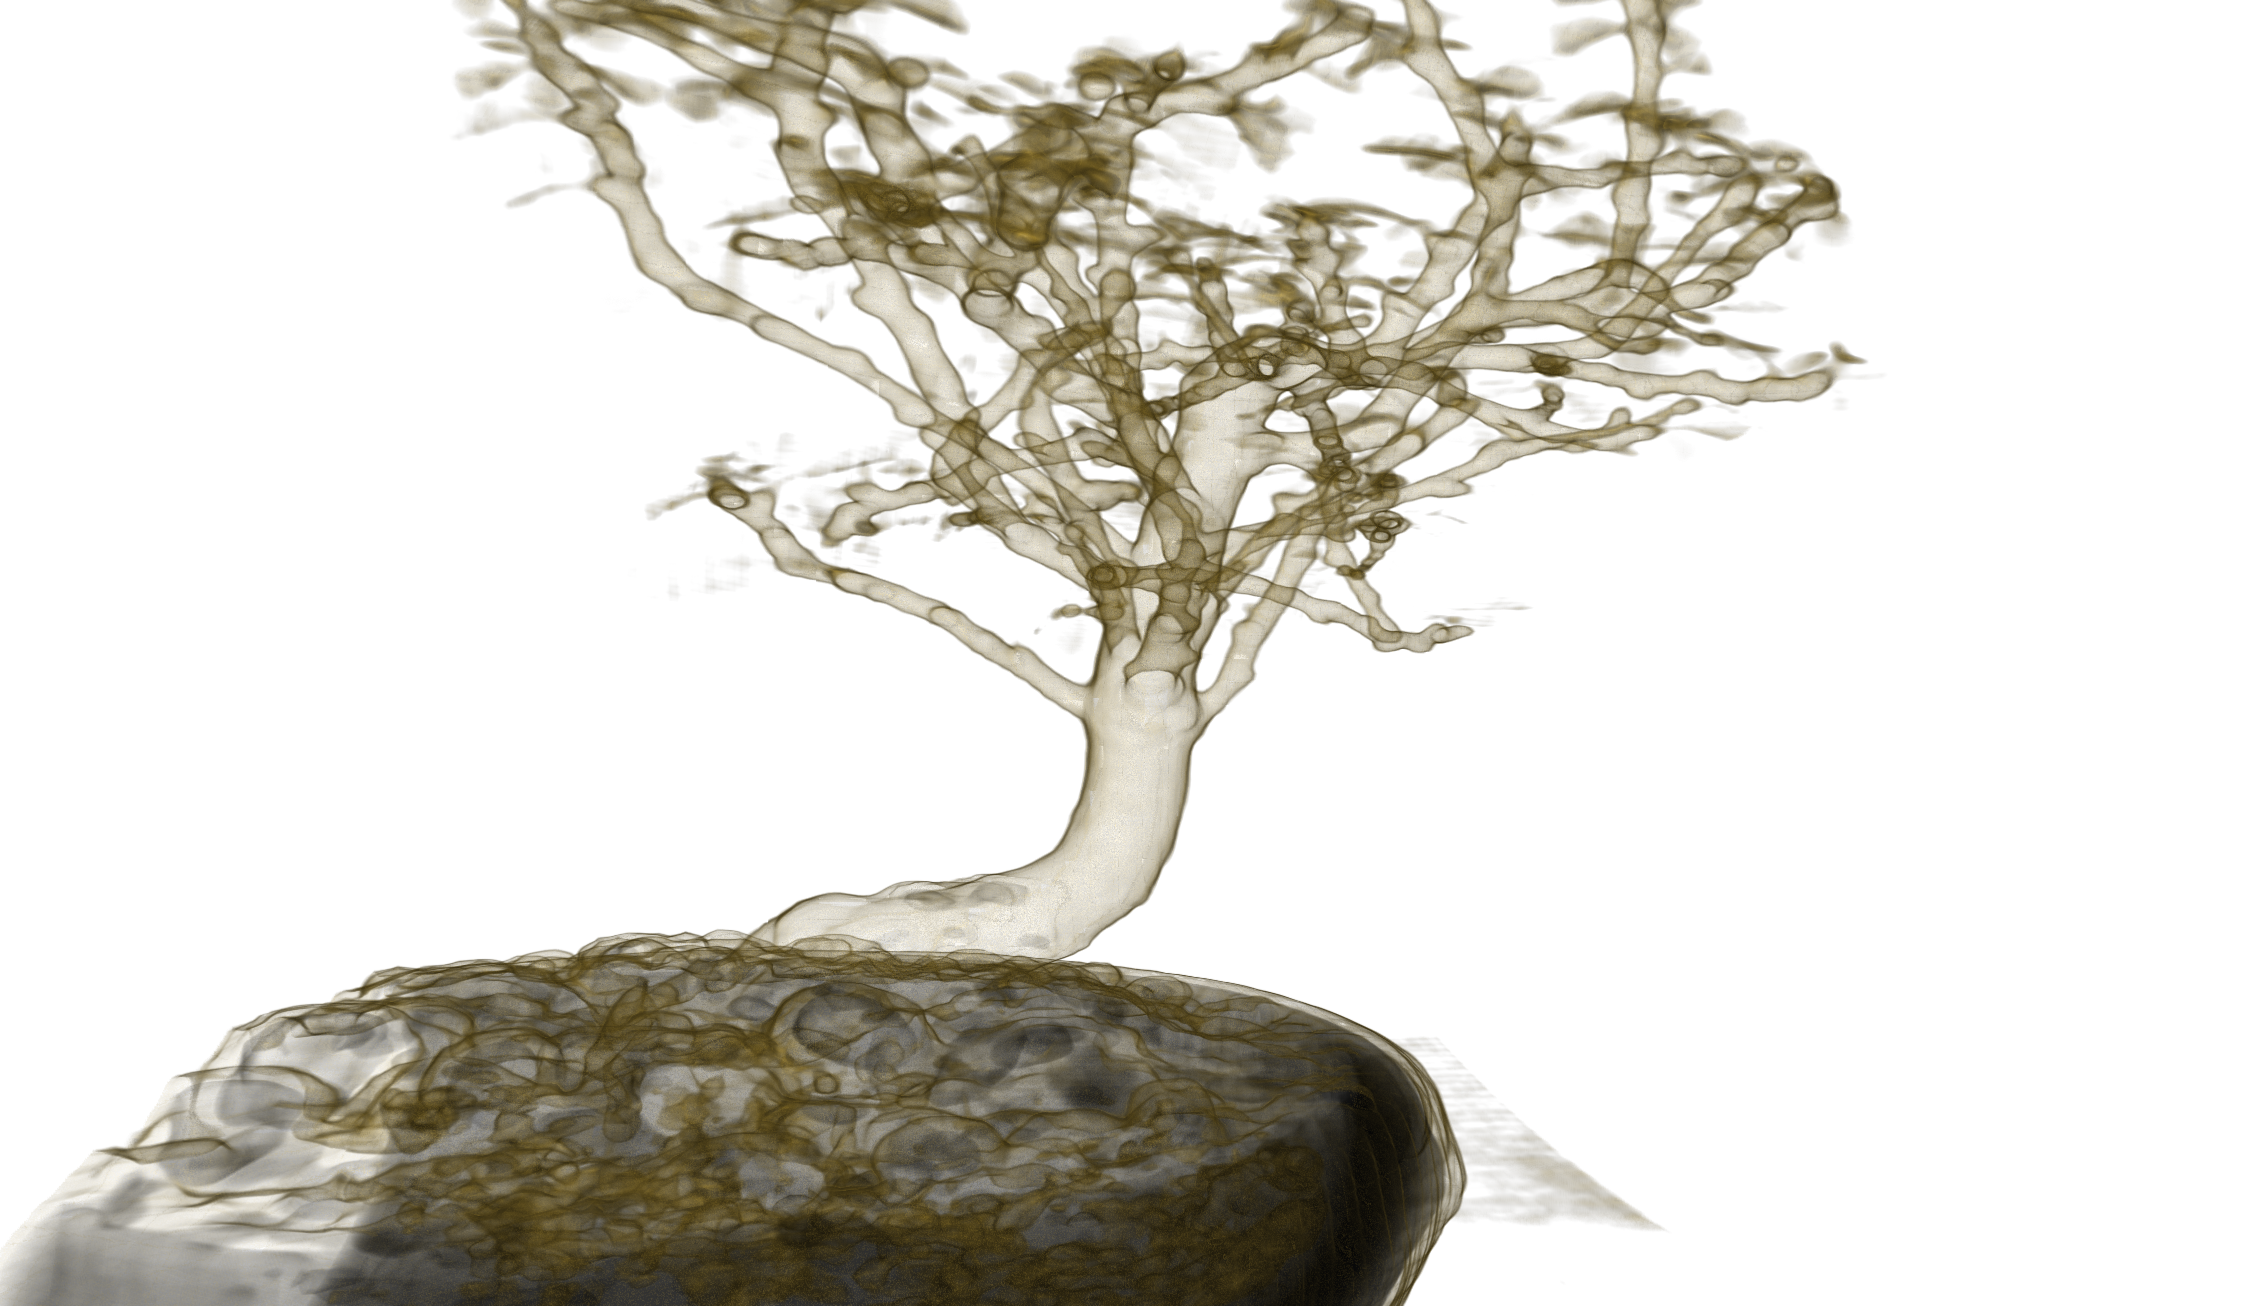
\includegraphics[width=\textheight]{../../Grafiken/results/picture_quality/bonsai/Standard_img-1_Ray-1-5.png}
		\caption{Volumen Bonsai mit ursprünglichem Raycast berechnet.}
		\label{fig::res::bon_st}
	\end{figure}
\end{landscape}

\begin{landscape}
	\begin{figure}
		\centering
		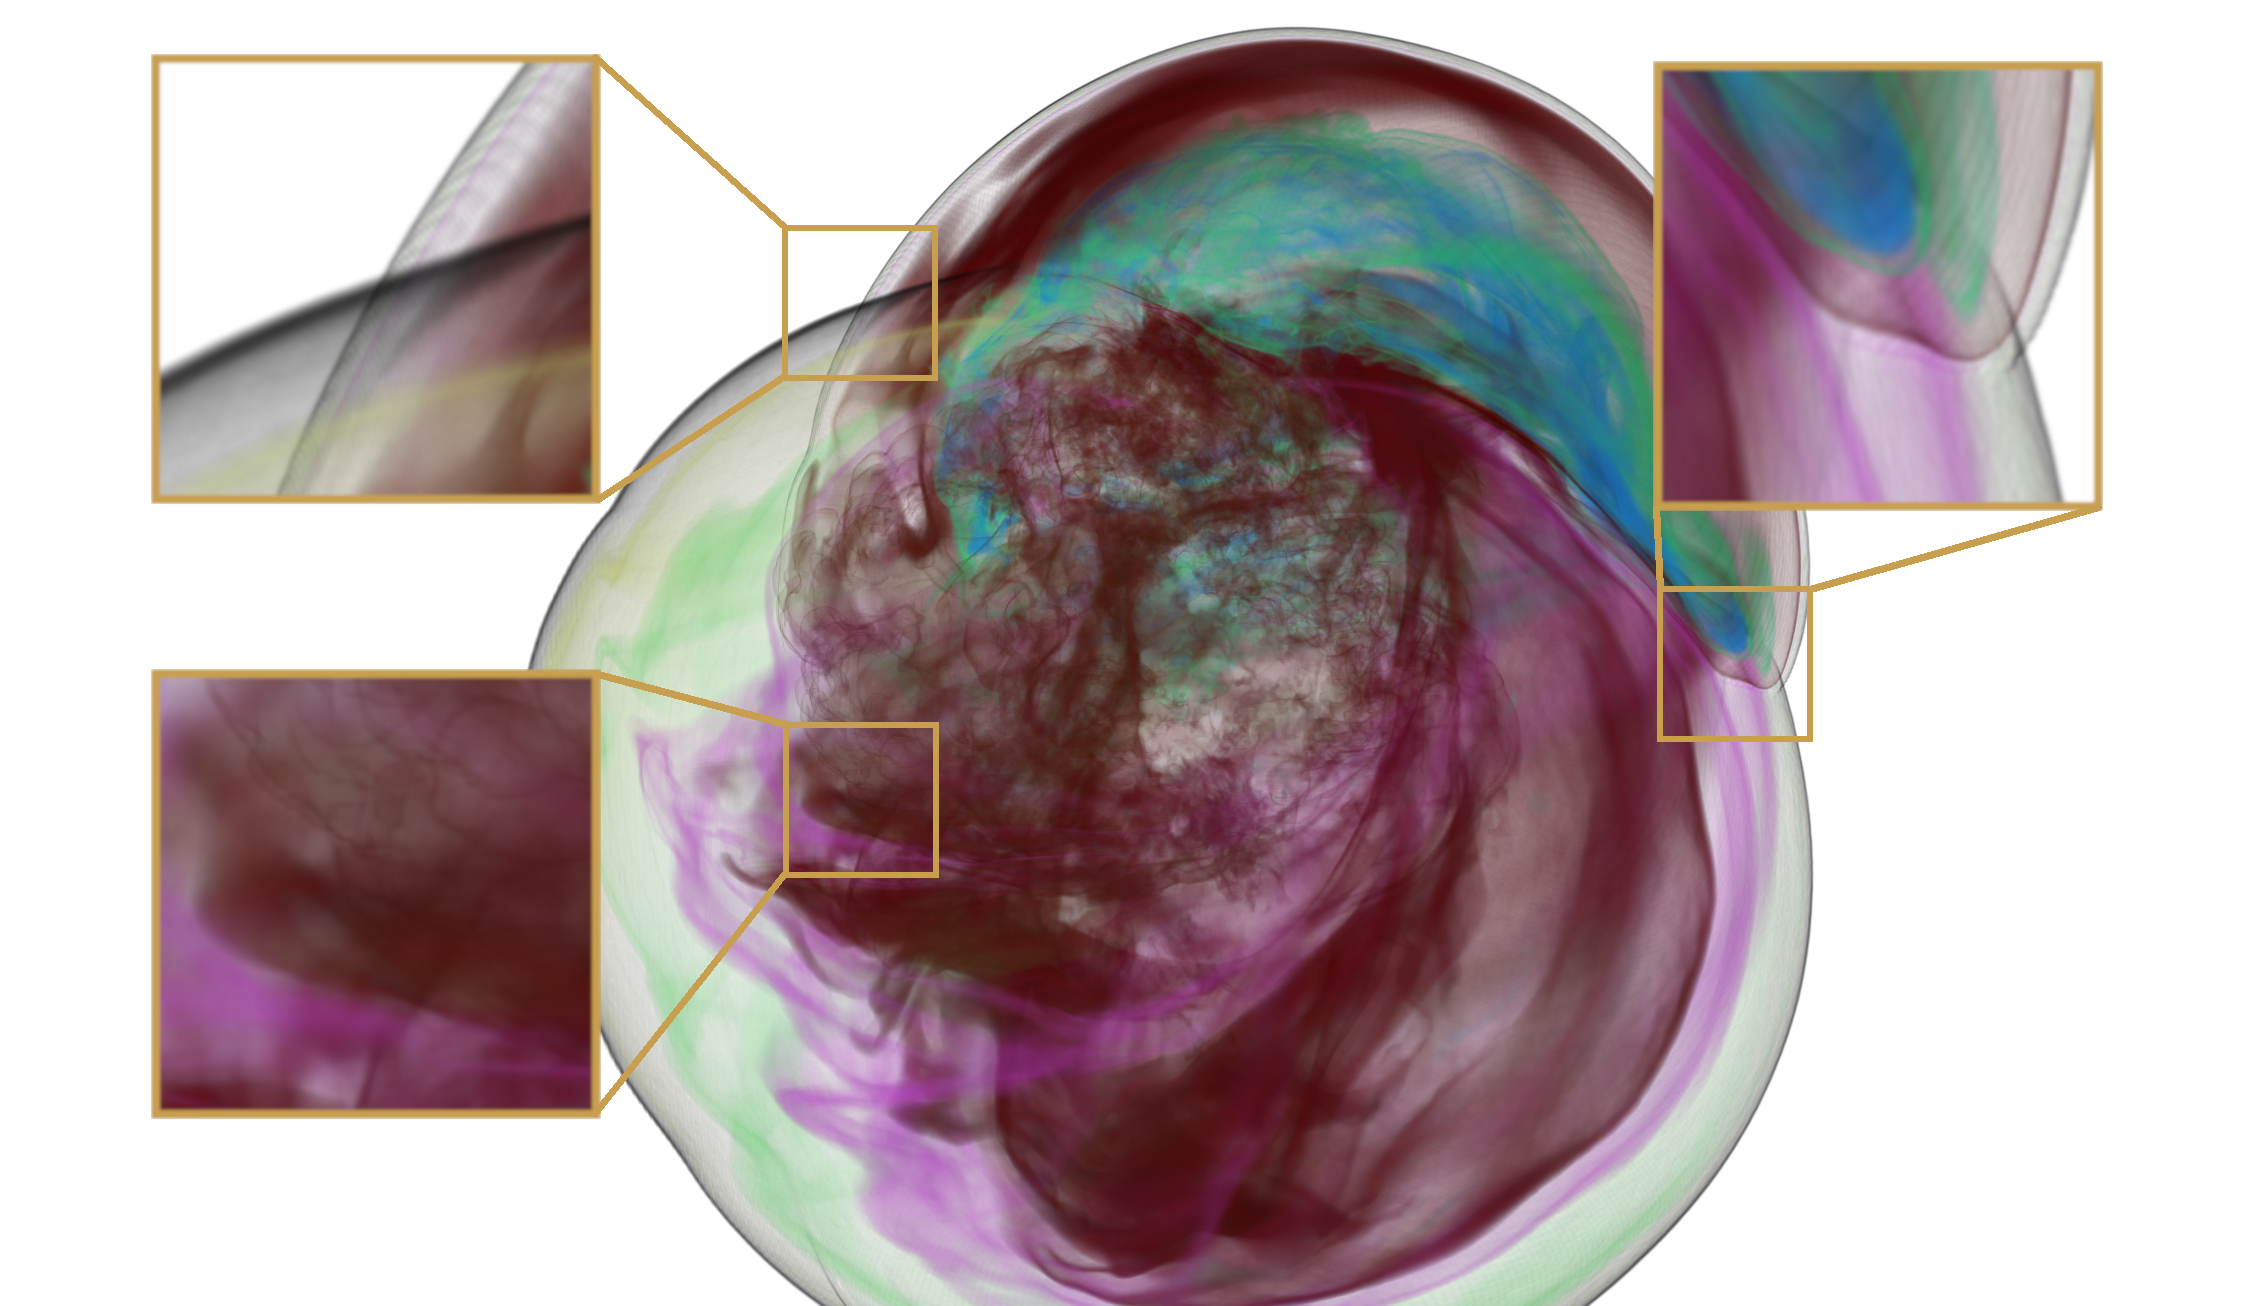
\includegraphics[width=\textheight]{../../Grafiken/results/picture_quality/supernova/Standard_img-1_Ray-1-5_edited.png}
		\caption{Volumen Supernova mit ursprünglichem Raycast berechnet und verschiedene Abschnitte vergrößert und hervorgehoben.}
		\label{fig::res::sup_st}
	\end{figure}
\end{landscape}

\subsubsection{MDC Raycast}\label{ss::res::mdc}
Der \emph{MDC} Raycast ist das Ergebnis des Arbeitspakets, aus dem Abschnitt \ref{ss::MDC}.
Die Abbildung \ref{fig::res::bon_mdc} zeigt das Volumen \emph{Bonsai}, welches mit dem \emph{MDC} Raycast erstellt wurde.
Das Bild wurde dabei aus der selben Perspektive und mit der gleichen Transferfunktion berechnet, wie dies auch in Abbildung \ref{fig::res::bon_st} der Fall war.
Die Strahlabtastrate ist ebenfalls gleich wie bei der Berechnung des Bildes in Abbildung \ref{fig::res::bon_st}, welches mit dem Standard Raycast berechnet wurde.
Die maximale Bildabtastrate in Abbildung \ref{fig::res::bon_mdc} hat einen Wert von $0.96$ statt einem Wert von $1$.
Damit wird einer leichten Verschiebung des Bildes, aufgrund der zwei unterschiedlichen Bildabtastraten, entgegengewirkt.
Die Anpassung der Bildabtastrate muss aber je nach Auflösung des Bildes leicht variiert werden.

In diesem Fall, beim \emph{MDC} Raycast, wurden zwei Bilder berechnet, welche anschließend passend zusammengefügt wurden.
Das erste Bild wurde mit nur einem viertel der Auflösung berechnet und anschließend auf die ursprüngliche Auflösung interpoliert.
Das zweite Bild wurde mit der ursprünglichen Auflösung berechnet, dafür aber nur ein rechteckiger Ausschnitt an der Mausposition.
Anschließend wurde das zweite Bild an der Mausposition in das auf die normale Auflösung interpolierte erste Bild eingefügt.

\todo{Mausposition in das Bild einzeichnen.}
An den Konturen der Abbildung \ref{fig::res::bon_mdc} ist ein leichter Abfall der Auflösung des Bildes zu erkennen.
Die Konturen, welche in Abbildung \ref{fig::res::bon_st} noch weich gezeichnet wurden, haben außerhalb des Rechtecks um die Mausposition nun Artefakte der Unterabtastung, wie zum Beispiel leichte Treppenstufen.
Innerhalb des Rechtecks sind die Konturen immer noch weich gezeichnet und es ist dort kein Unterschied zu Abbildung \ref{fig::res::bon_st} zu sehen.

Die Größe des Rechtecks beträgt $300$\,Pixel in x- und y-Richtung und ist groß genug, dass die Abnahme der Auflösung im äußeren Bereich kaum auffällt.
Wird bei aktivem Eyetracking anstelle der Mausposition die Blickposition verwendet, so ist der aktuell betrachtete Bereich immer hoch aufgelöst.
Ein Unterschied zwischen den beiden Bereichen fällt während einer Fokussierung kaum auf.
Wenn der Fokus langsam über das Bild wandert, kann man einen Unterschied zwischen den Auflösungen erkennen.
An dem Übergang des normal aufgelösten Bereichs zu dem Bereich mit der halben Auflösung kommt es während einer Bewegung an den Konturen des Volumen zu leichten Veränderungen.
Diese können die Aufmerksamkeit auf sich ziehen und daher leicht störend wirken.

Obwohl der Bereich außerhalb des Rechtecks mit nur einem Viertel der Bildabtastrate innerhalb des Rechtecks berechnet wurde, ist die Bildqualität in diesem Bereich noch recht gut.
Da die Sehschärfe mit zunehmenden Winkel von der Fovea weg immer weiter abnimmt, könnte die Bildabtastrate außerhalb des Rechtecks vermutlich weiter gesenkt werden, ohne dass dies die Bildqualität bei der Verwendung eines Eye-Trackers beeinträchtigt.

Das Bild in Abbildung \ref{fig::res::sup_mdc} wurde ebenfalls mit dem \emph{MDC} Raycast berechnet und anschließend bearbeitet.
Es zeigt einen Zeitschritt in einer Simulation von einer Supernova.
Die Bild- und Strahlabtastrate ist gleich wie zuvor in Abbildung \ref{fig::res::bon_mdc}.
Die Mausposition ist hier als nicht ganz ausgefüllter Kreis skizziert.
In der Abbildung \ref{fig::res::sup_mdc} sind drei Bildausschnitte des berechneten Bildes, innerhalb des Rechtecks, außerhalb des Rechtecks und an der Kante des Rechtecks, vergrößert, um diese besser vergleichen zu können.
Rechts über der skizzierten Mausposition ist ein Ausschnitt des Übergangs zwischen den Auflösungen, welcher rechts davon vergrößert dargestellt ist.
Man kann erkennen, dass die Konturen des Objekt außerhalb des Rechtecks unschärfer sind.
Unterhalb der skizzierten Mausposition ist zuerst ein Ausschnitt innerhalb des Rechtecks mit normaler Bildabtastrate und darunter ein Ausschnitt außerhalb des Rechtecks mit nur einem viertel der Auflösung vergrößert.
In dem unterem Ausschnitt wirken die Konturen insgesamt ein bisschen unschärfer und verwaschen.
Der Unterschied fällt aber nicht sehr stark auf.

% Die Latenz des Eyetrackers ist sehr gut. ; Perf.
% Eine merkbare Verzögerung zwischen realer Blickposition und der Blickposition des aktuell berechneten Bildes, tritt nur dann auf, falls die Berechnungsdauer eines Bildes zu lange dauert. ; Perf
% Dies hängt aber auch von der Größe und Auflösung des verwendeten Volumens ab. ; Perf.
% In dem Fall von Abbildung \ref{fig::res::bon_st} ist dies nicht der Fall. ; Perf.
% Da das Volumen mit einer Auflösung von $256\times256\times256$\,Voxel im Vergleich zu anderen recht klein ist, .. ; Perf.
\begin{landscape}
	\begin{figure}
		\centering
		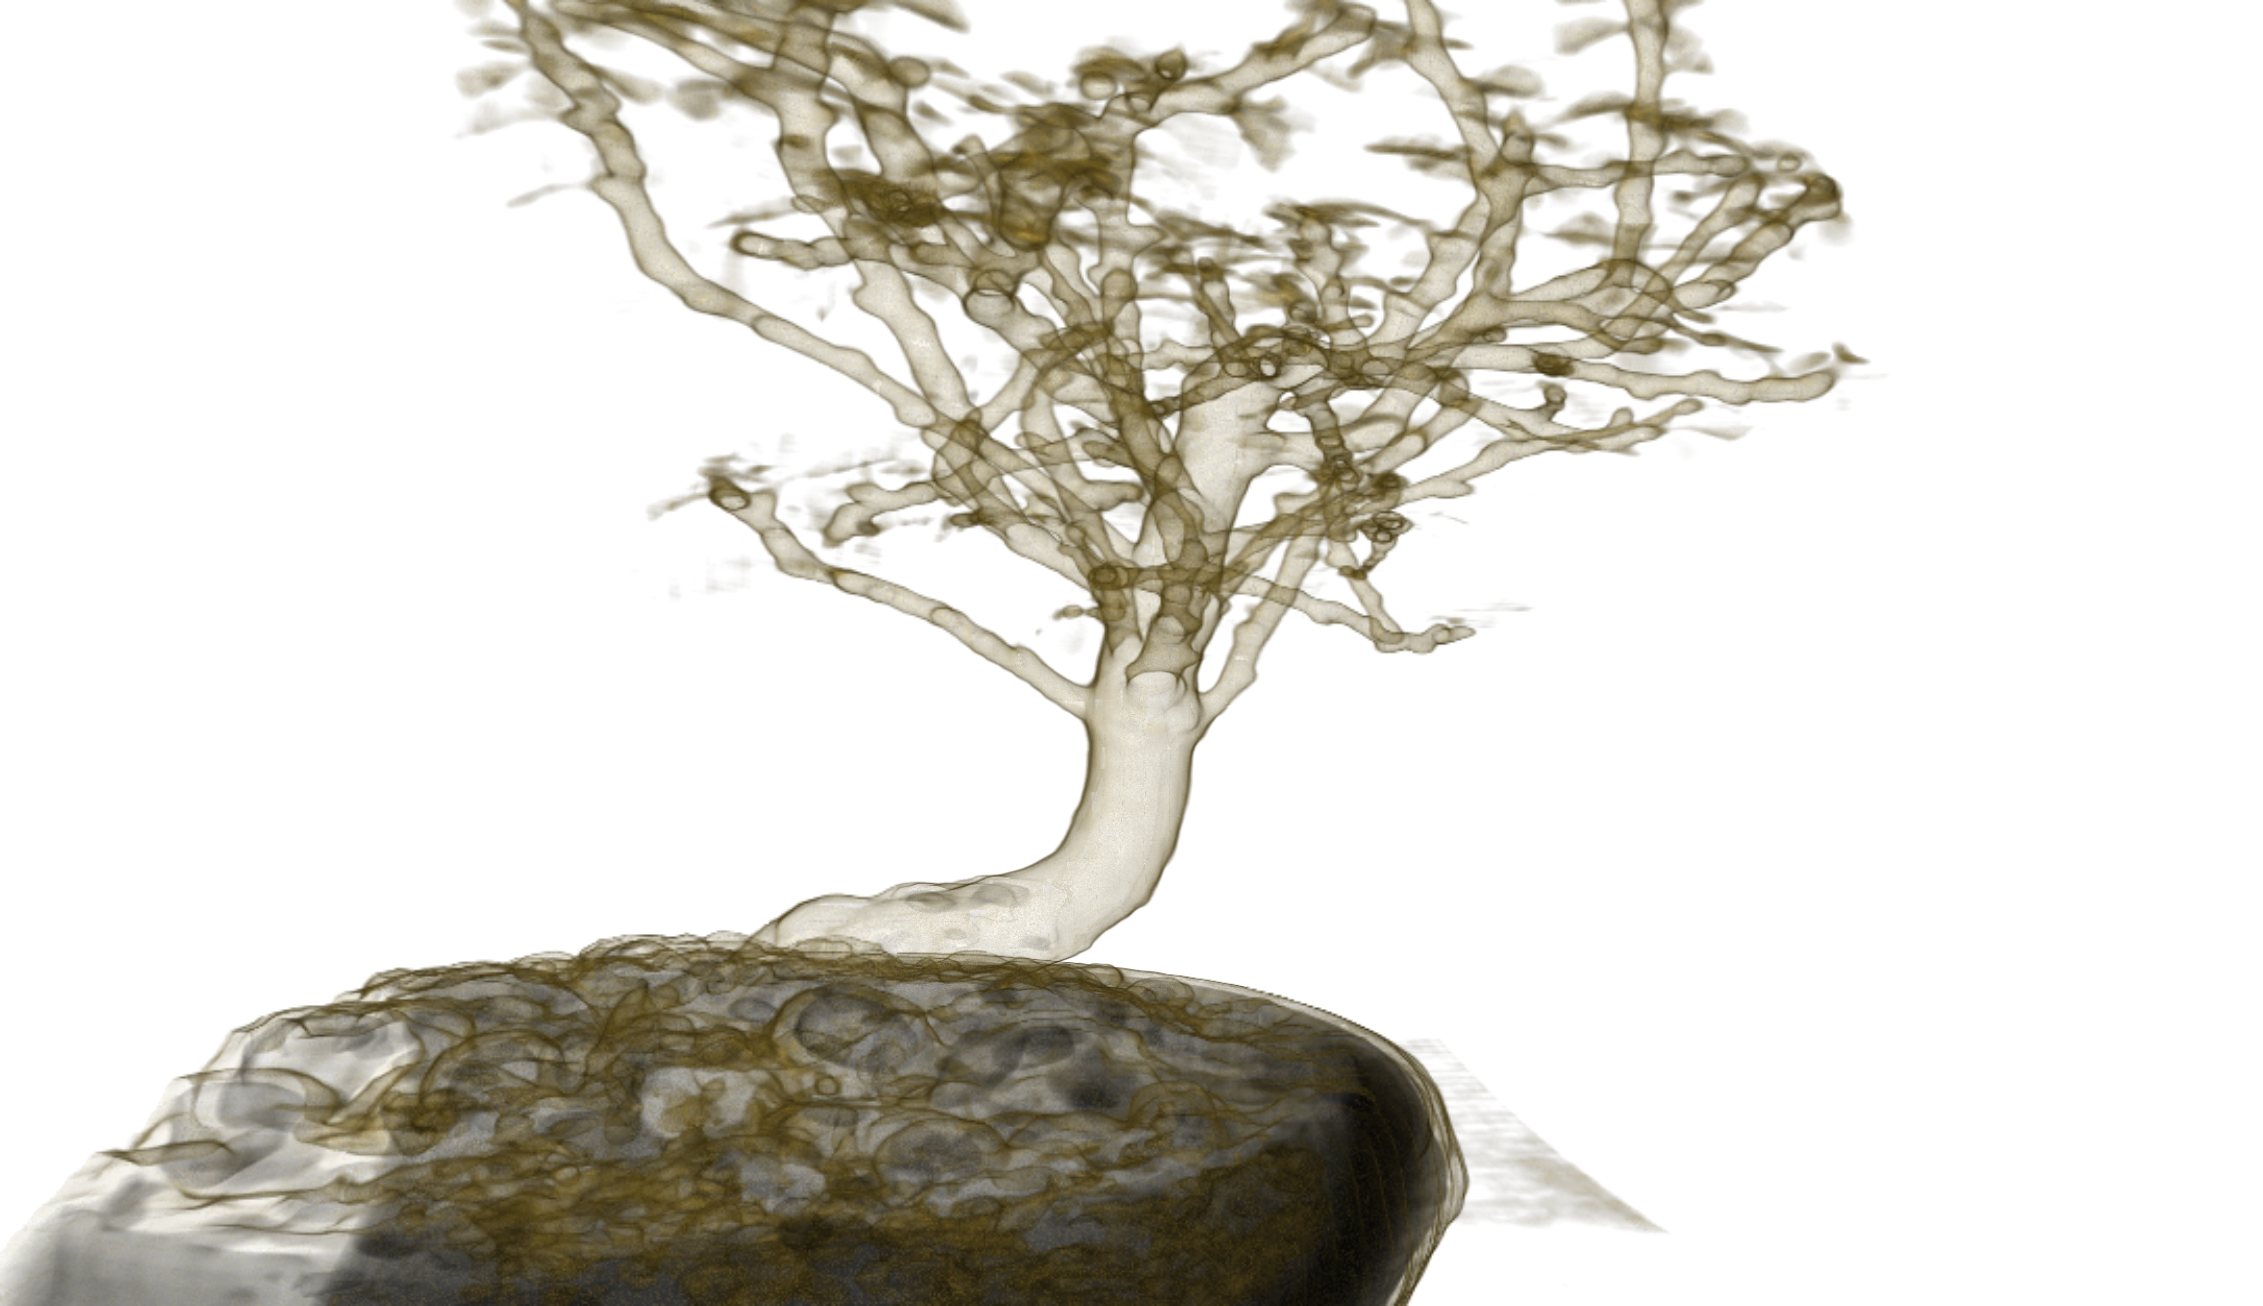
\includegraphics[width=1\textheight]{../../Grafiken/results/picture_quality/bonsai/MDC_img-0-96_ray-1-5.png}
		\caption{Volumen Bonsai mit \emph{MDC} Raycast berechnet.}
		\label{fig::res::bon_mdc}
	\end{figure}
\end{landscape}

\begin{landscape}
	\begin{figure}
		\centering
		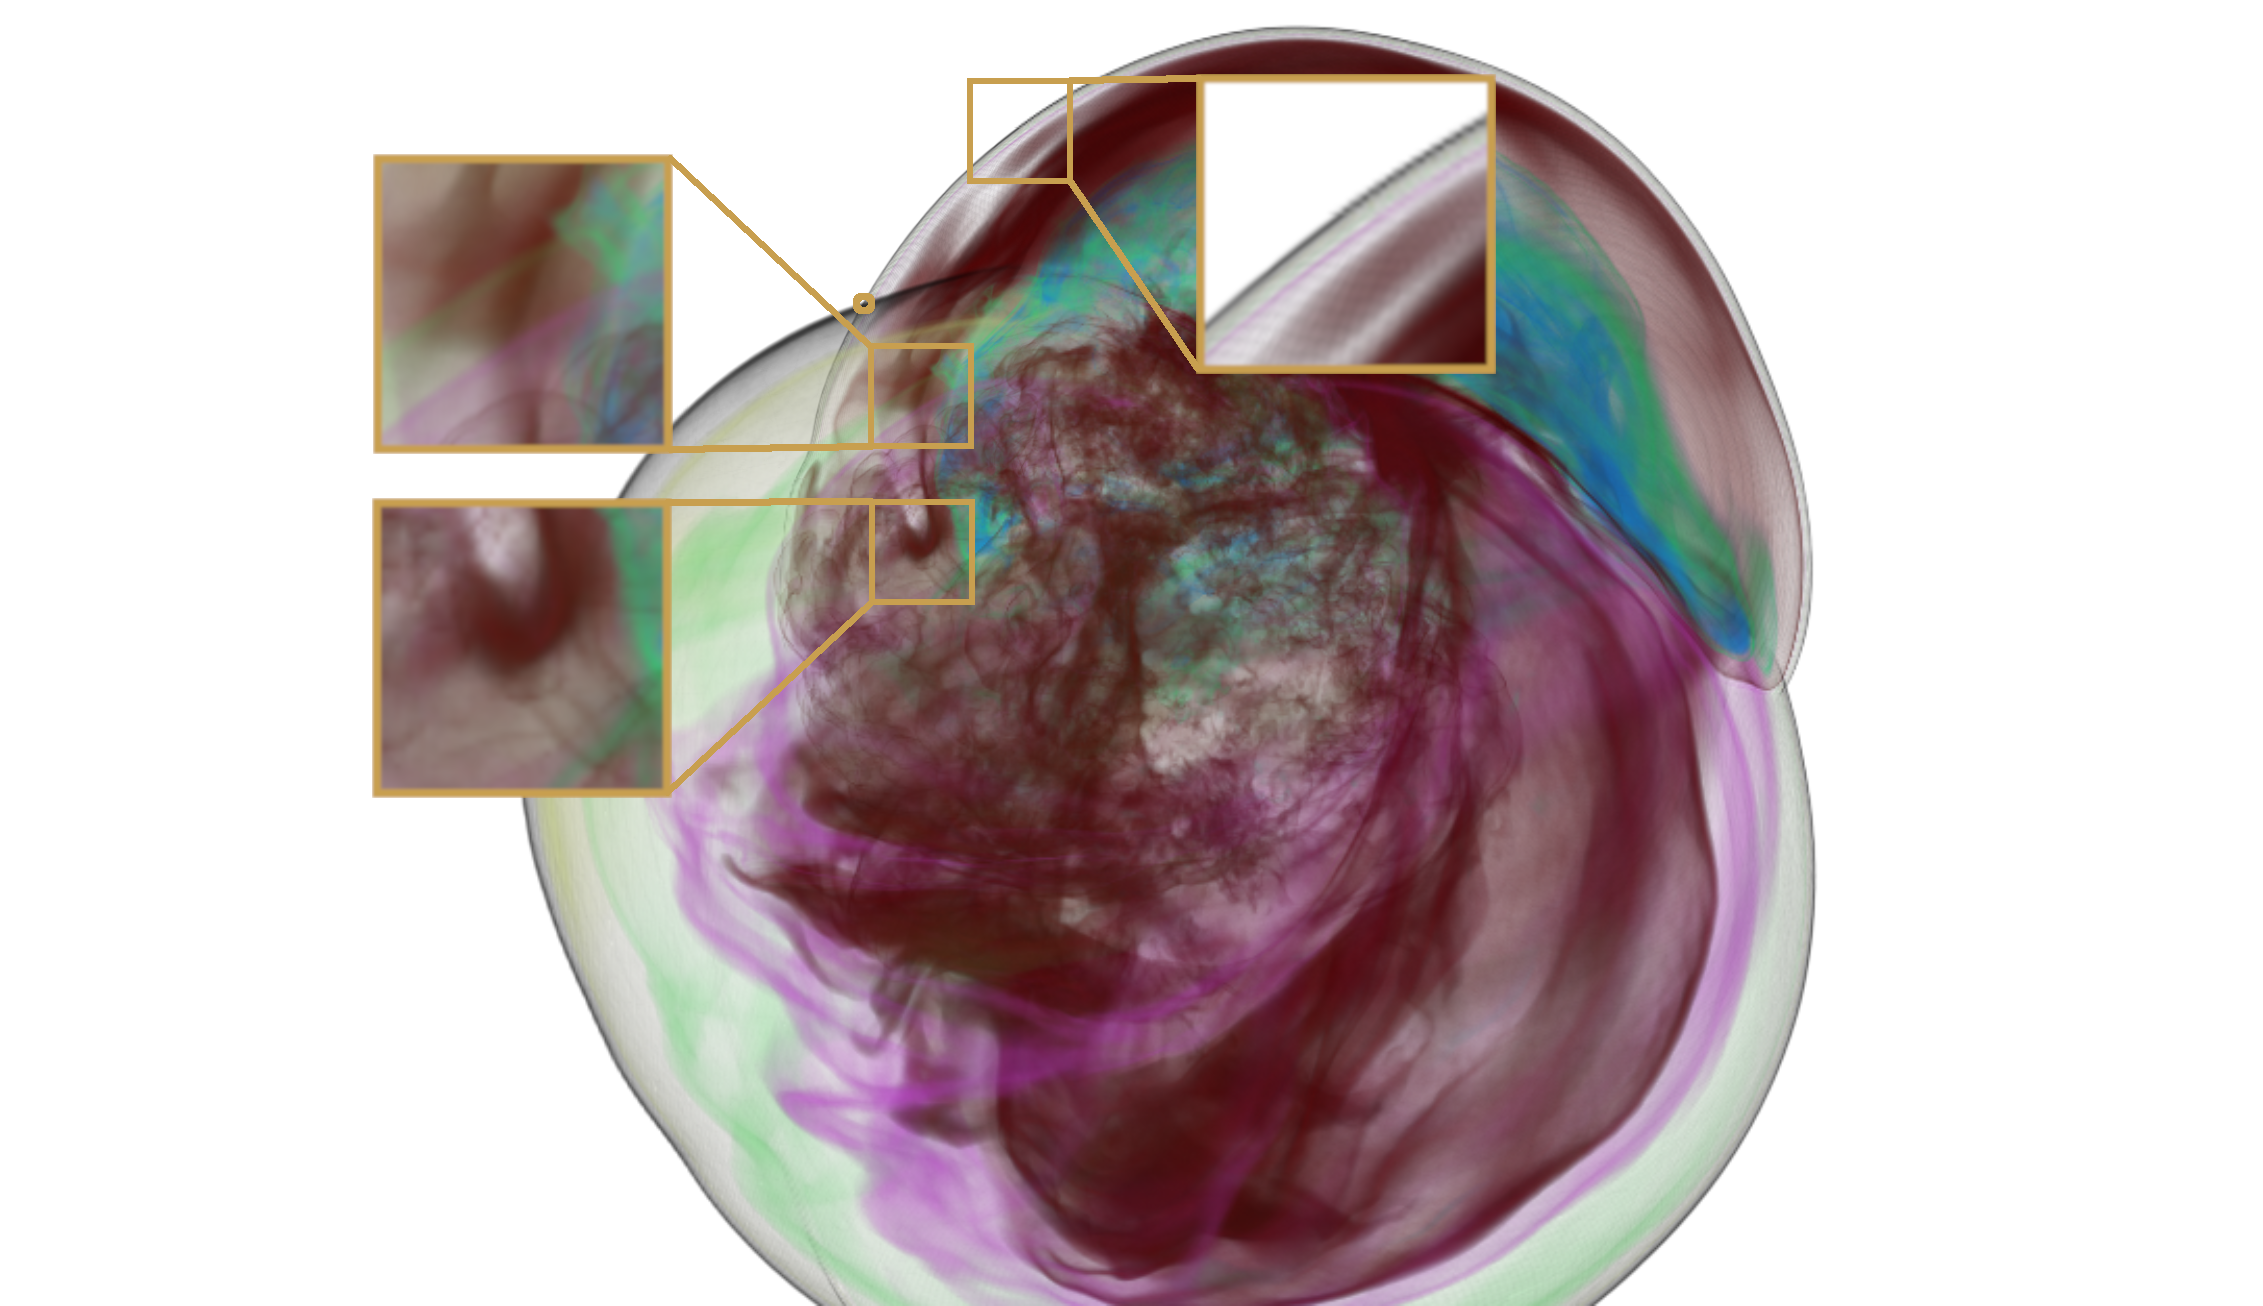
\includegraphics[width=\textheight]{../../Grafiken/results/picture_quality/supernova/MDC_img-0-96_ray-1-5_edited.png}
		\caption{Volumen Supernova mit \emph{MDC} Raycast berechnet mit vergrößerten Bildausschnitten.}
		\label{fig::res::sup_mdc}
	\end{figure}
\end{landscape}

\subsubsection{DDC Raycast}\label{ss::res::ddc}
Der \emph{DDC} Raycast ist das Ergebnis des Arbeitspakets aus dem Abschnitt \ref{ss::DDC}.
Abbildung \ref{fig::res::bon_ddc} zeigt das Volumen \emph{Bonsai}, welches mit dem \emph{DDC} Raycast erstellt wurde.
Das Bild wurde aus der selben Perspektive und mit der gleichen Transferfunktion berechnet, wie in den Abbildungen \ref{fig::res::bon_st} und \ref{fig::res::bon_mdc}.
Anders als beim Standard Raycast und \emph{MDC} Raycast, wo die Strahlabtastrate über das gesamte Bild hinweg gleich ist, nimmt beim \emph{DDC} Raycast die Strahlabtastrate Abhängig zur Distanz eines Strahls zur Maus- beziehungsweise Blickposition ab.
In einem kleinen Bereich um die Mausposition hat sie den maximalen Wert, der gleich dem Wert aus \emph{MDC} und dem Standard Raycast ist.
Die maximale Bildabtastrate ist $1$.
Diese nimmt in zwei Stufen nach außen hin ab.

Beim \emph{DDC} Raycast wurde nur ein Aufruf des Raycasts gestartet und die Work-Items und ihre entsprechenden Strahlen auf verschiedene Bildpunkte abgebildet.
Das gesamte Bild wurde in einem zweiten Kernel Aufruf interpoliert.
Innerhalb eines kleinen Bereichs in der Form einer Ellipse um den Blickpunkt herum hat das Bild eine Bildabtastrate von $1$, dass heißt jeder Pixel entspricht einem Farbwert der Auswertung eines Strahls.
Außerhalb von diesem Bereich aber innerhalb einer zweiten größeren und umschließenden Ellipse hat das Bild in x- und y-Richtung eine Bildabtastrate von $\frac{1}{2}$.
Das heißt, dass in x- und y-Richtung nur für jedes zweiten Pixel ein Strahl ausgewertet wird.
In dem äußersten Bereich beträgt die Bildabtastrate in x- und y-Richtung $\frac{1}{7}$.
Es wird also in jedem $7\times7$\,Pixel-Feld nur ein Strahl ausgewertet.

In Abbildung \ref{fig::res::bon_ddc} ist deutlich zu sehen, dass der Großteil des Bildes eine geringe Auflösung hat.
In dem am niedrigsten abgetasteten Bereich sind an den Konturen, insbesondere die der Äste, deutliche Merkmale der Unterabtastung zu sehen.
In Abbildung \ref{fig::res::bon_st} und \ref{fig::res::bon_mdc} verlaufen die Konturen der Äste noch diagonal und sind relativ weich gezeichnet, hier haben sie starke Treppeneffekte.

In dem mittleren Bereich ist die Bildqualität recht gut und die das Bild scharf zu erkennen.
Trotzdem hat das Bild hier nur ein Viertel der Auflösung.
Zwischen dem mittleren und inneren Bereich, welcher die normale Auflösung hat, ist kaum zu erkennen.

Dass die Strahlabtastrate mit zunehmender Entfernung zur Mausposition abnimmt, ist in Abbildung \ref{fig::res::bon_ddc} kaum zu erkennen.
Die reduzierte Auflösung verändert die Bildqualität im äußeren Bereich so stark, dass die reduzierte Strahlabtastrate nicht auffällt.

Abbildung \ref{fig::res::sup_ddc} zeigt das selbe Volumen wie in Abbildung \ref{fig::res::sup_st} und \ref{fig::res::sup_mdc}.
Bildausschnitte der Übergänge zwischen den Bereichen sind hier zur Verdeutlichung hervorgehoben und vergrößert.
Der vergrößerte Bildausschnitt rechts oben zeigt den Übergang zwischen dem mittleren und dem inneren Bereich.
Oben links ist der vergrößerte Übergang zwischen dem inneren und dem mittleren Bereich zu sehen.
Der Bildausschnitt unten links ist etwas größer und umfasst den Übergang von dem inneren zum mittleren und vom mittleren zum äußeren Bereich.

\begin{landscape}
	\begin{figure}
		\centering
		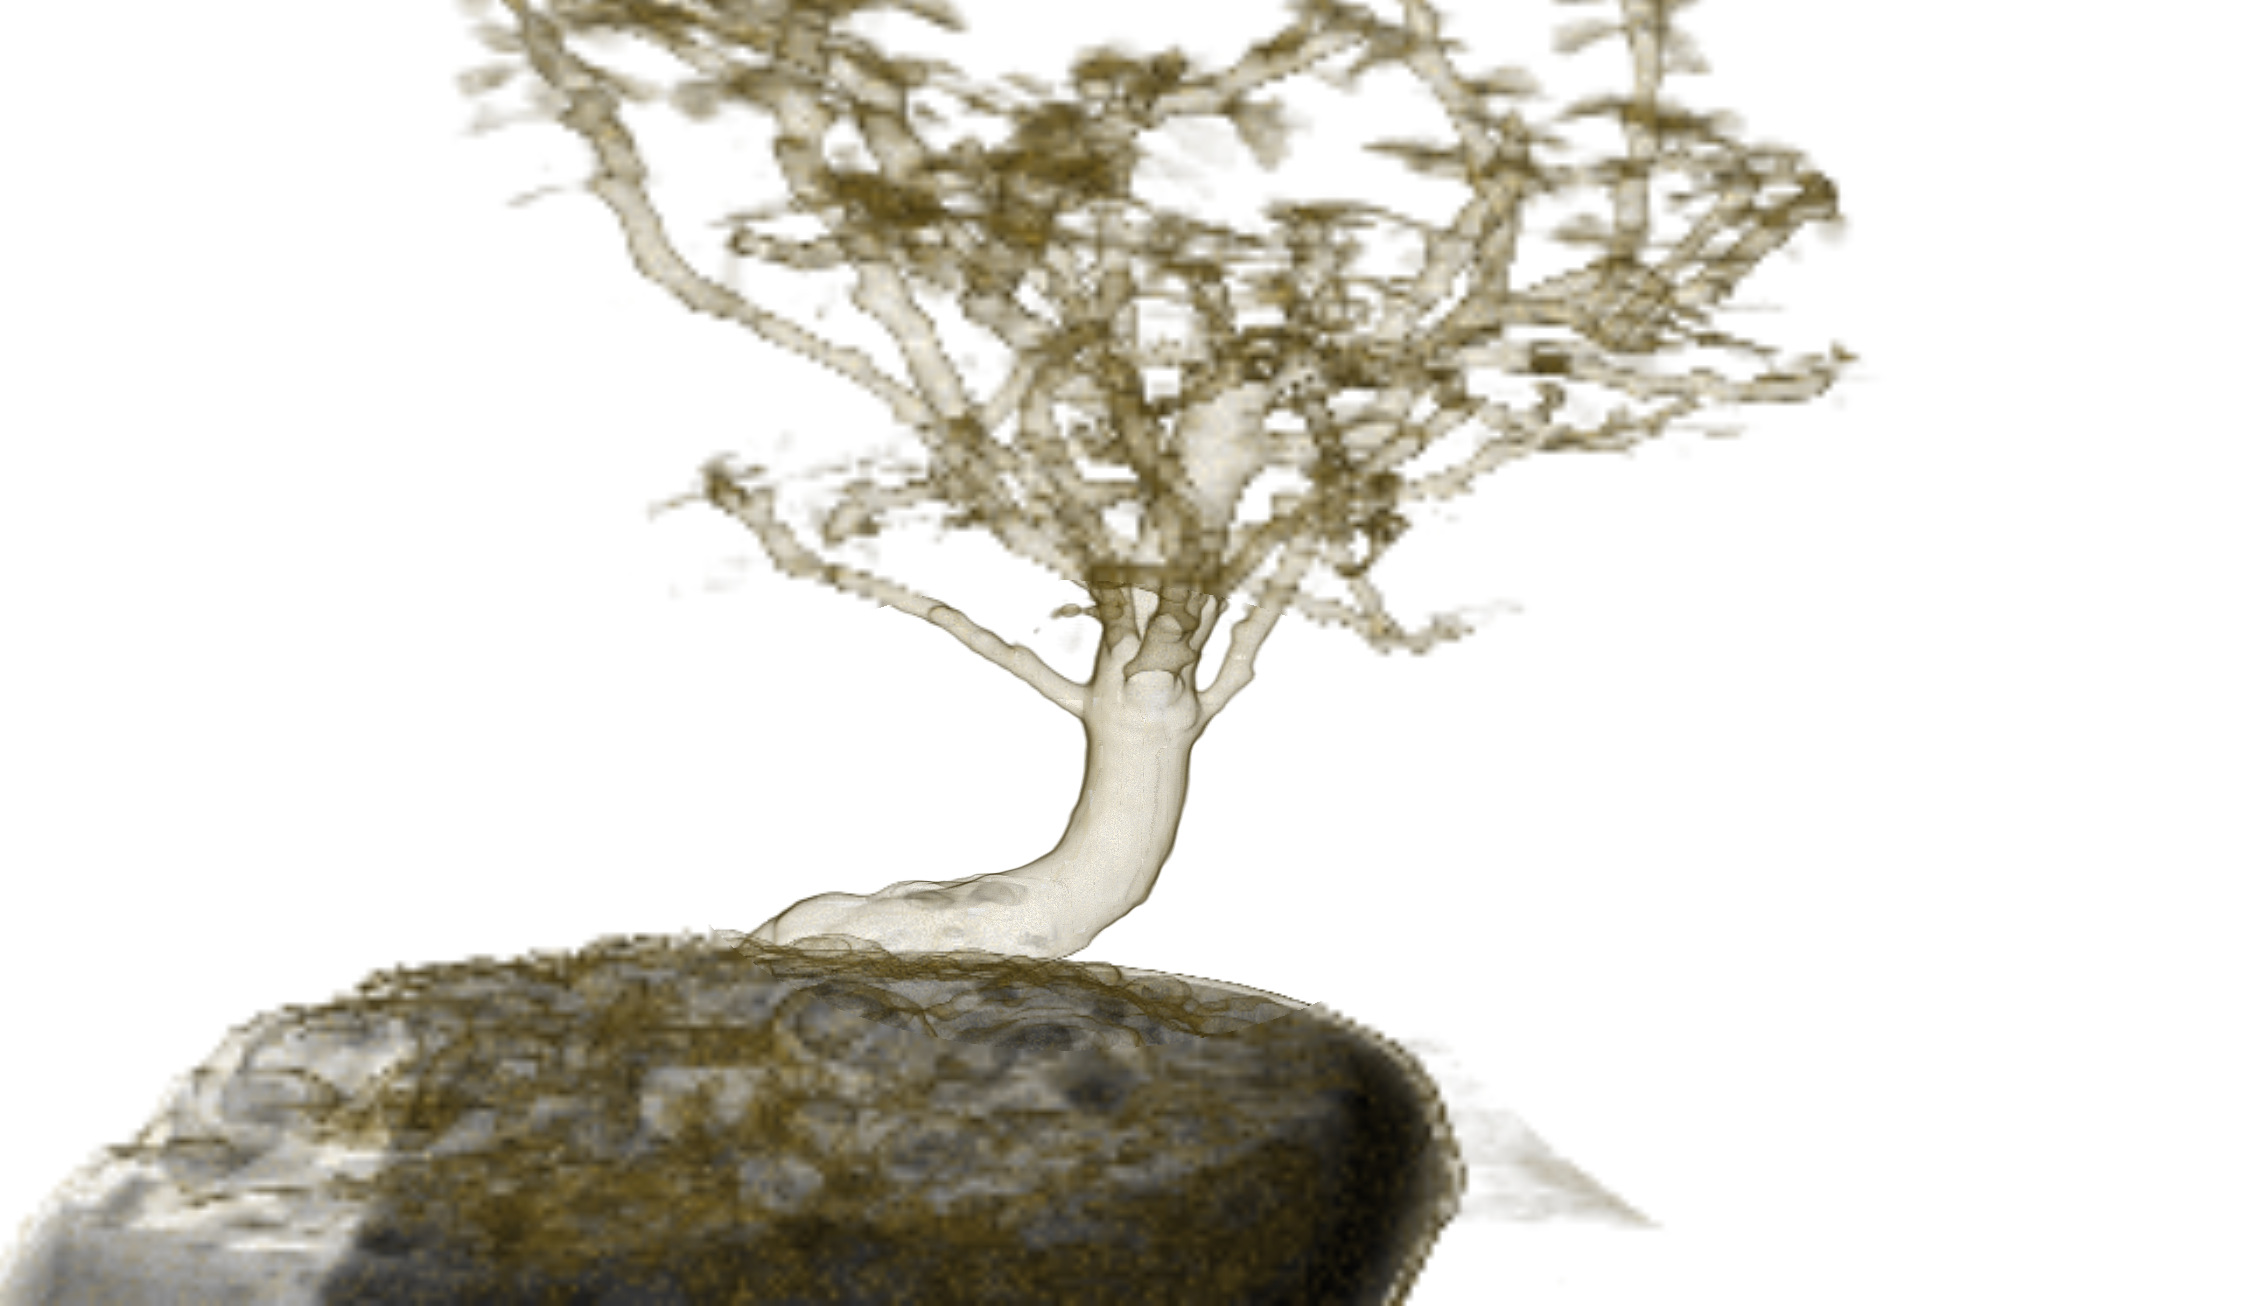
\includegraphics[width=1\textheight]{../../Grafiken/results/picture_quality/bonsai/DDC_img-1_ray-1-5.png}
		\caption{Volumen Bonsai mit \emph{DDC} Raycast berechnet mit.}
		\label{fig::res::bon_ddc}
	\end{figure}
\end{landscape}

\begin{landscape}
	\begin{figure}
		\centering
		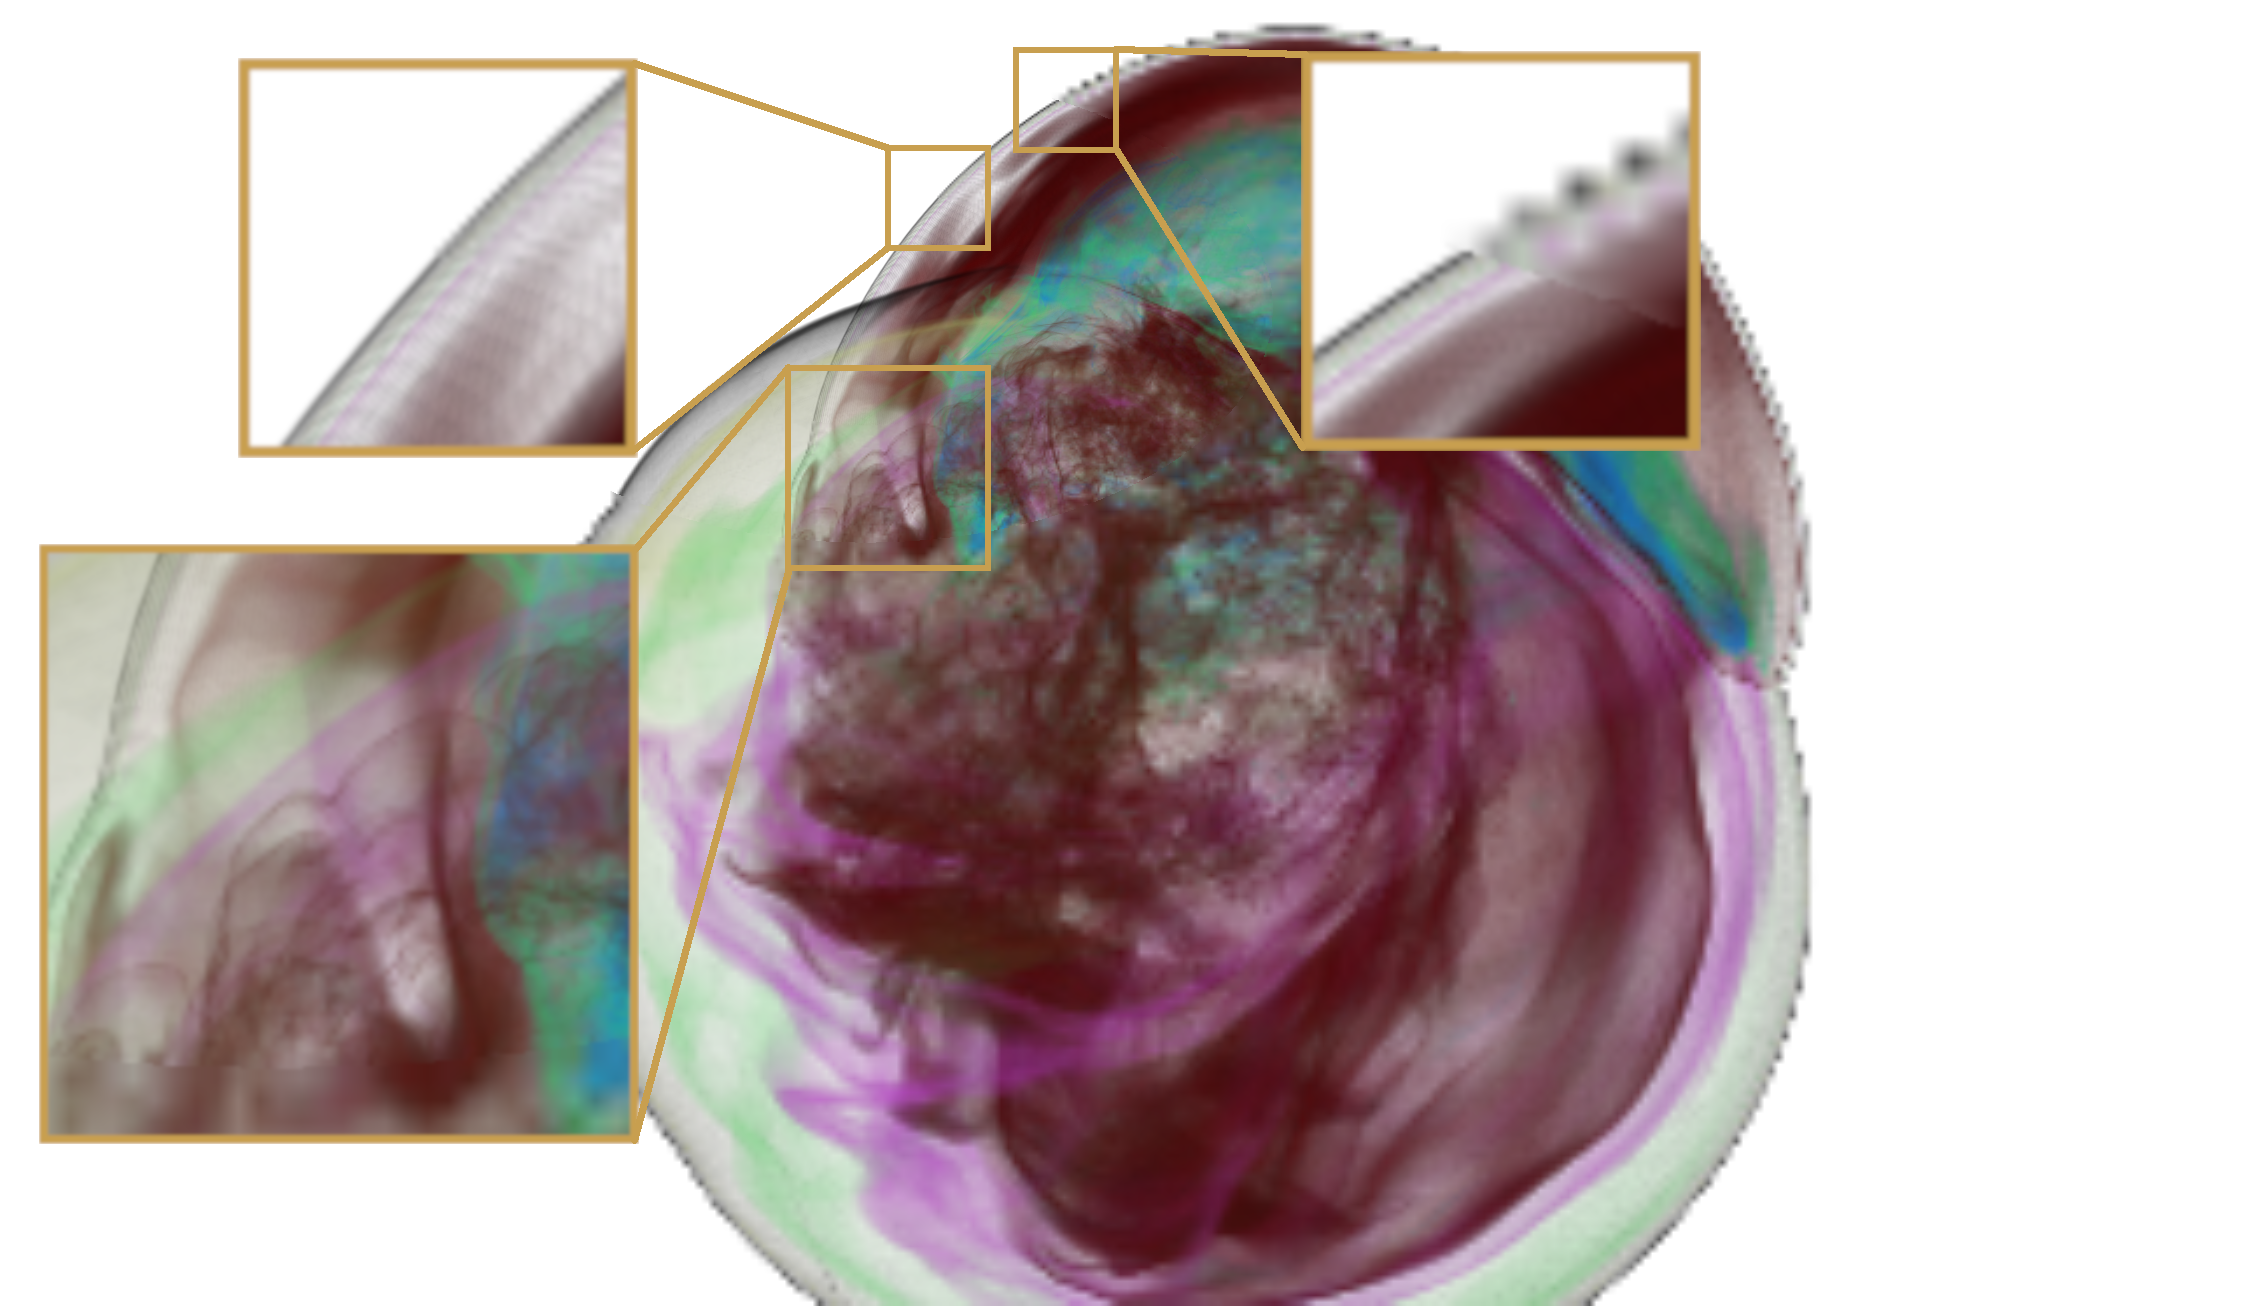
\includegraphics[width=\textheight]{../../Grafiken/results/picture_quality/supernova/DDC_img-1_ray-1-5_edited.png}
		\caption{Volumen Supernova mit \emph{DDC} Raycast berechnet mit hervorgehobenen und vergrößerten Bildausschnitten.}
		\label{fig::res::sup_ddc}
	\end{figure}
\end{landscape}

\iffalse




\begin{landscape}
	\begin{figure}
		\centering
		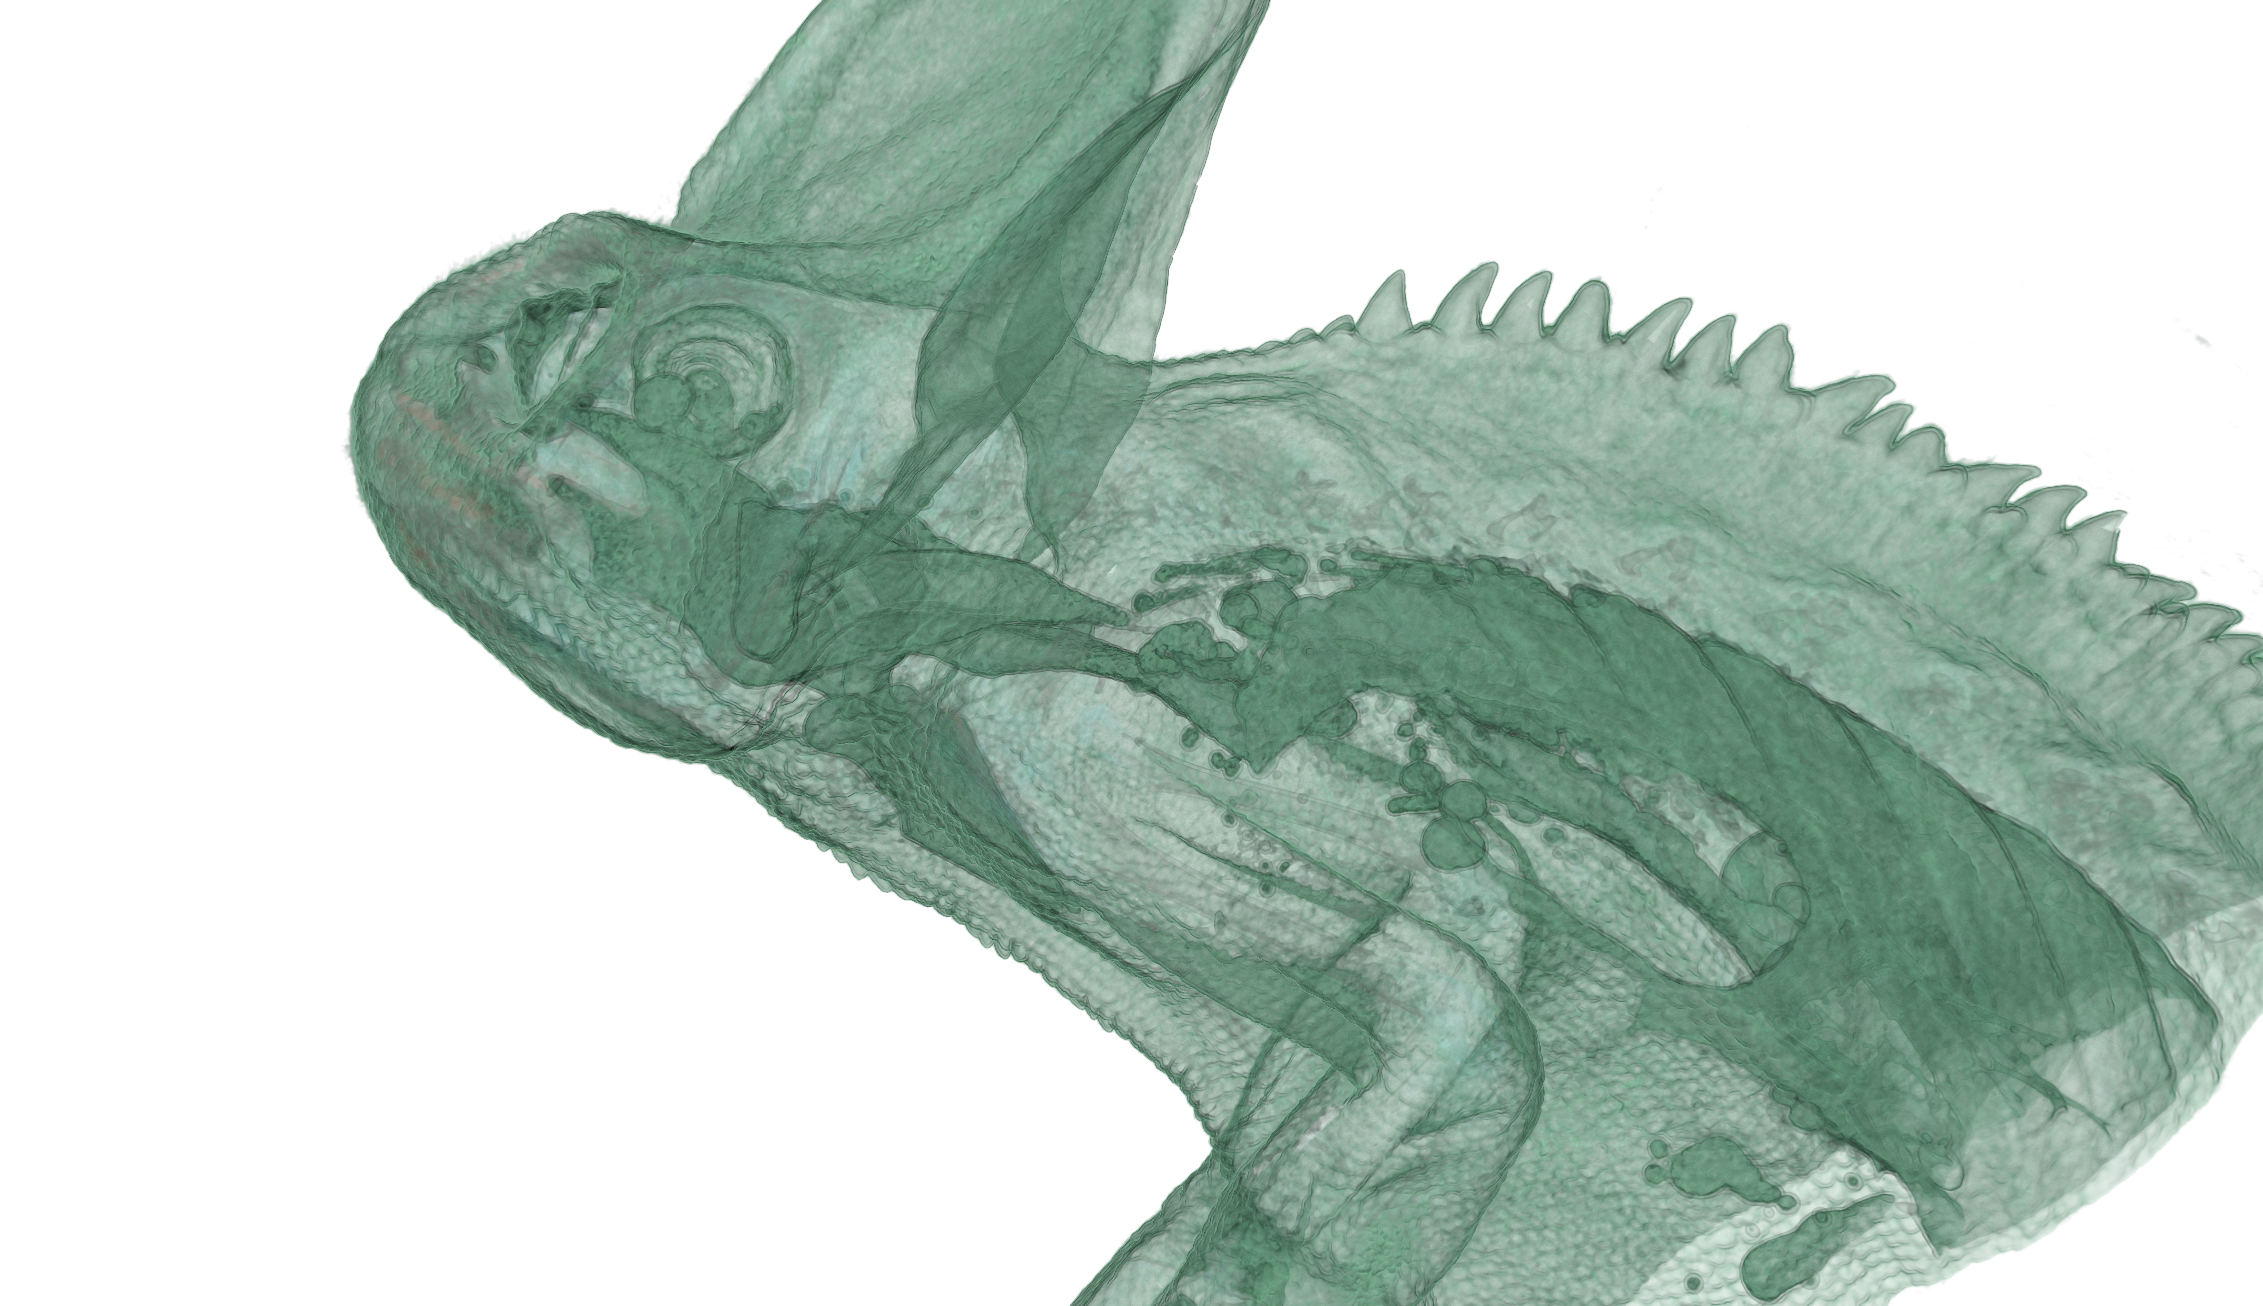
\includegraphics[width=1\textheight]{../../Grafiken/results/picture_quality/chameleon/Standard_img-1_Ray-1-5.png}
		\caption{Volumen Chameleon mit ursprünglichem Raycast berechnet.}
		\label{fig::res::cam_st}
	\end{figure}
\end{landscape}

\begin{landscape}
	\begin{figure}
		\centering
		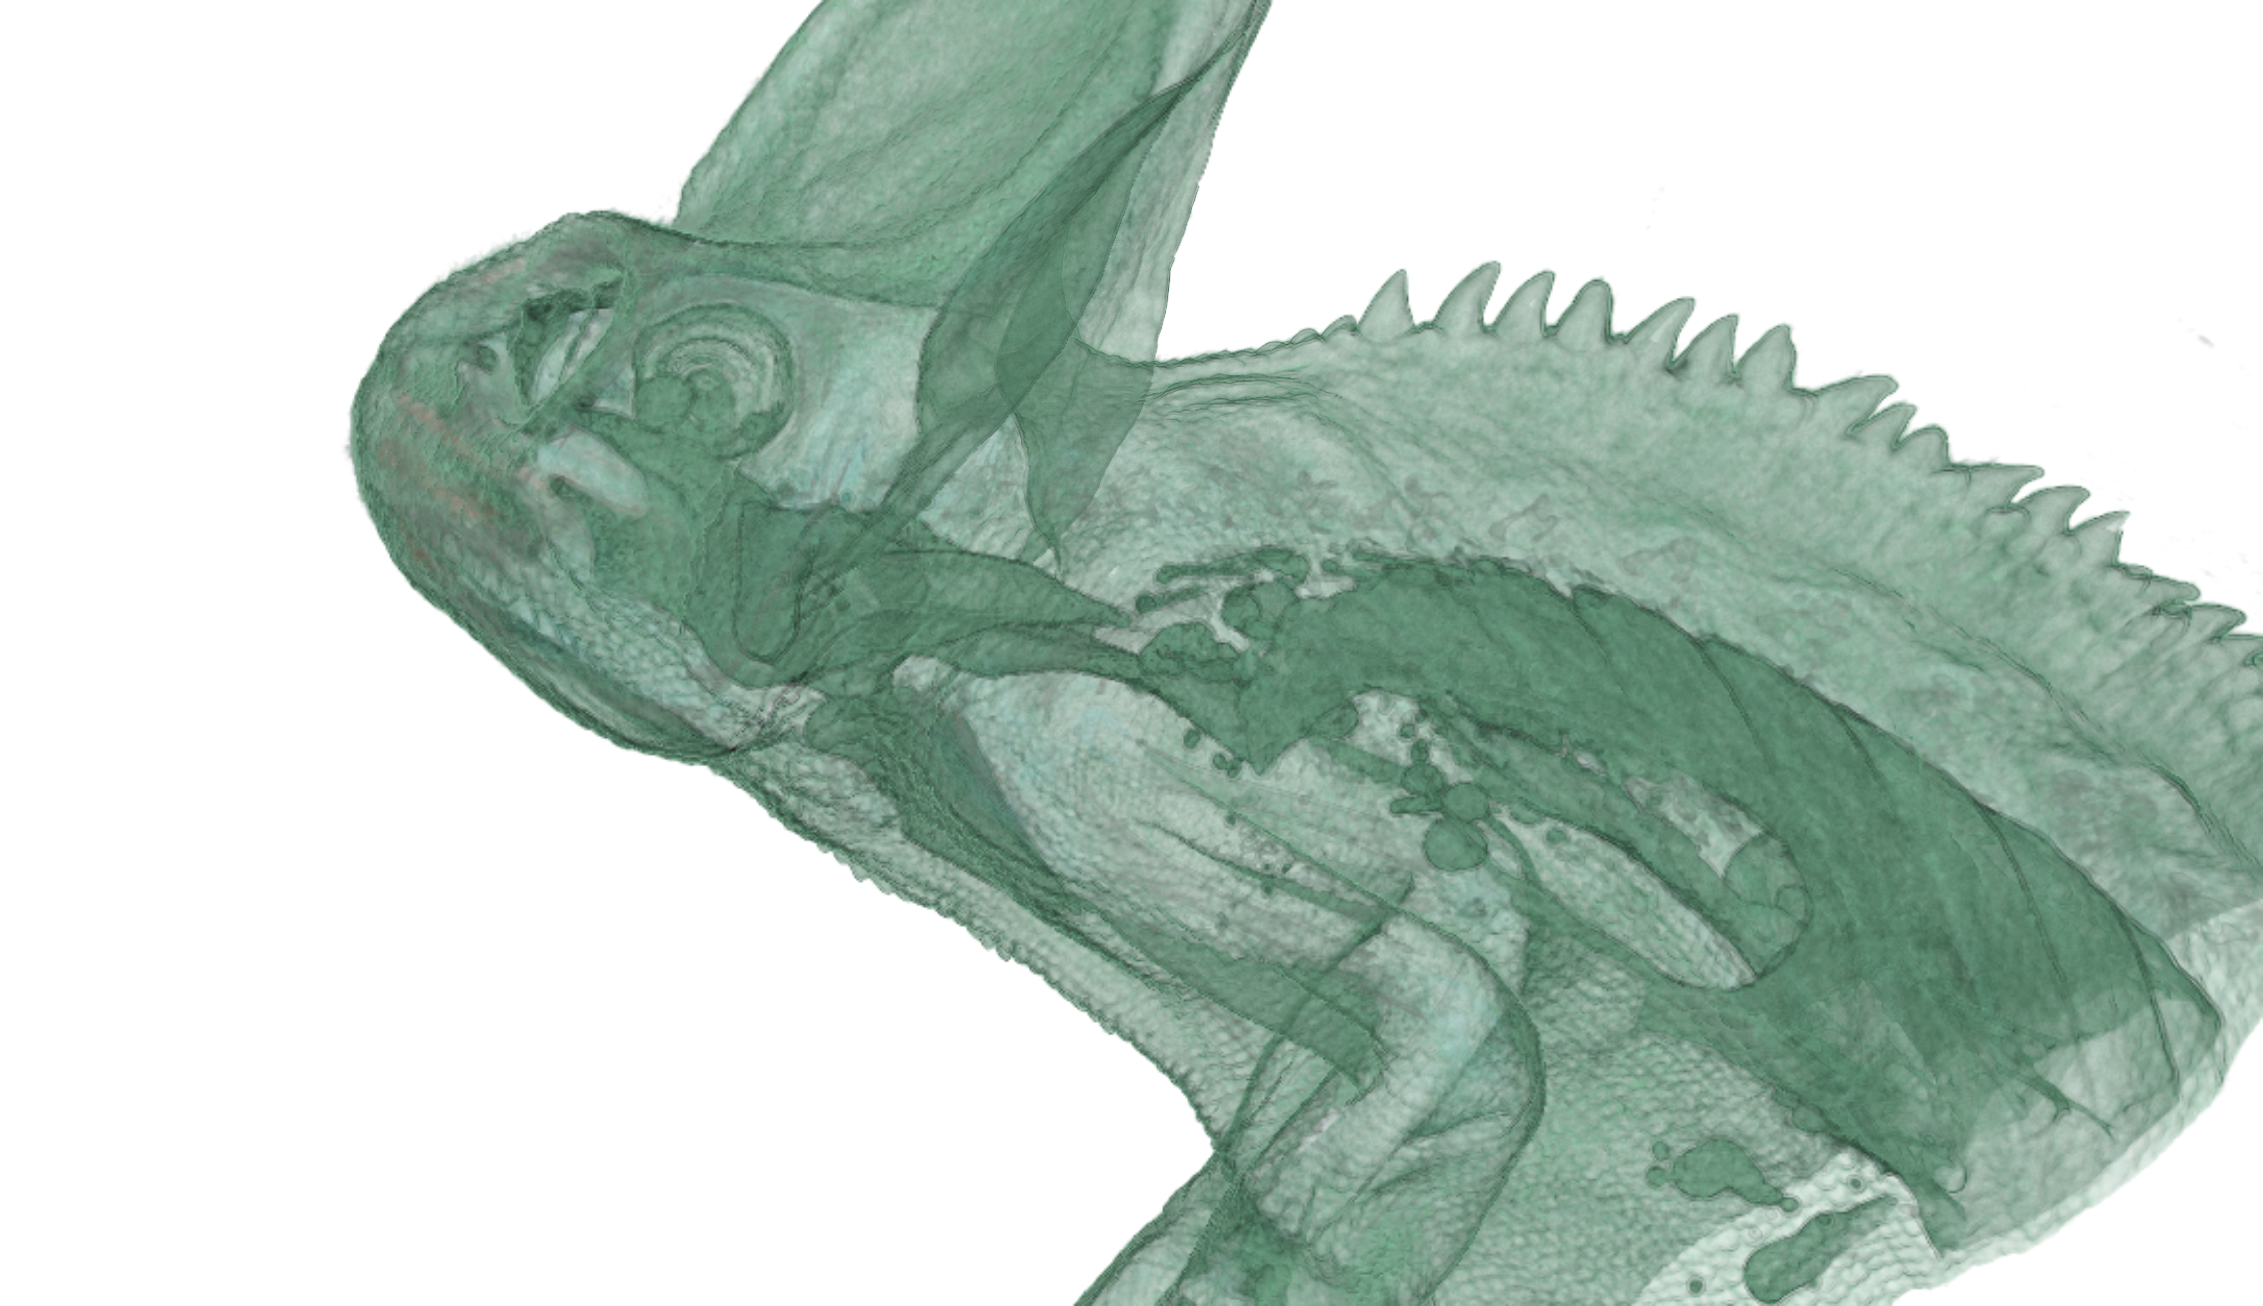
\includegraphics[width=1\textheight]{../../Grafiken/results/picture_quality/chameleon/MDC_img-0-96_ray-1-5.png}
		\caption{Volumen Chameleon mit \emph{MDC} Raycast berechnet.}
		\label{fig::res::cam_mdc}
	\end{figure}
\end{landscape}

\begin{landscape}
	\begin{figure}
		\centering
		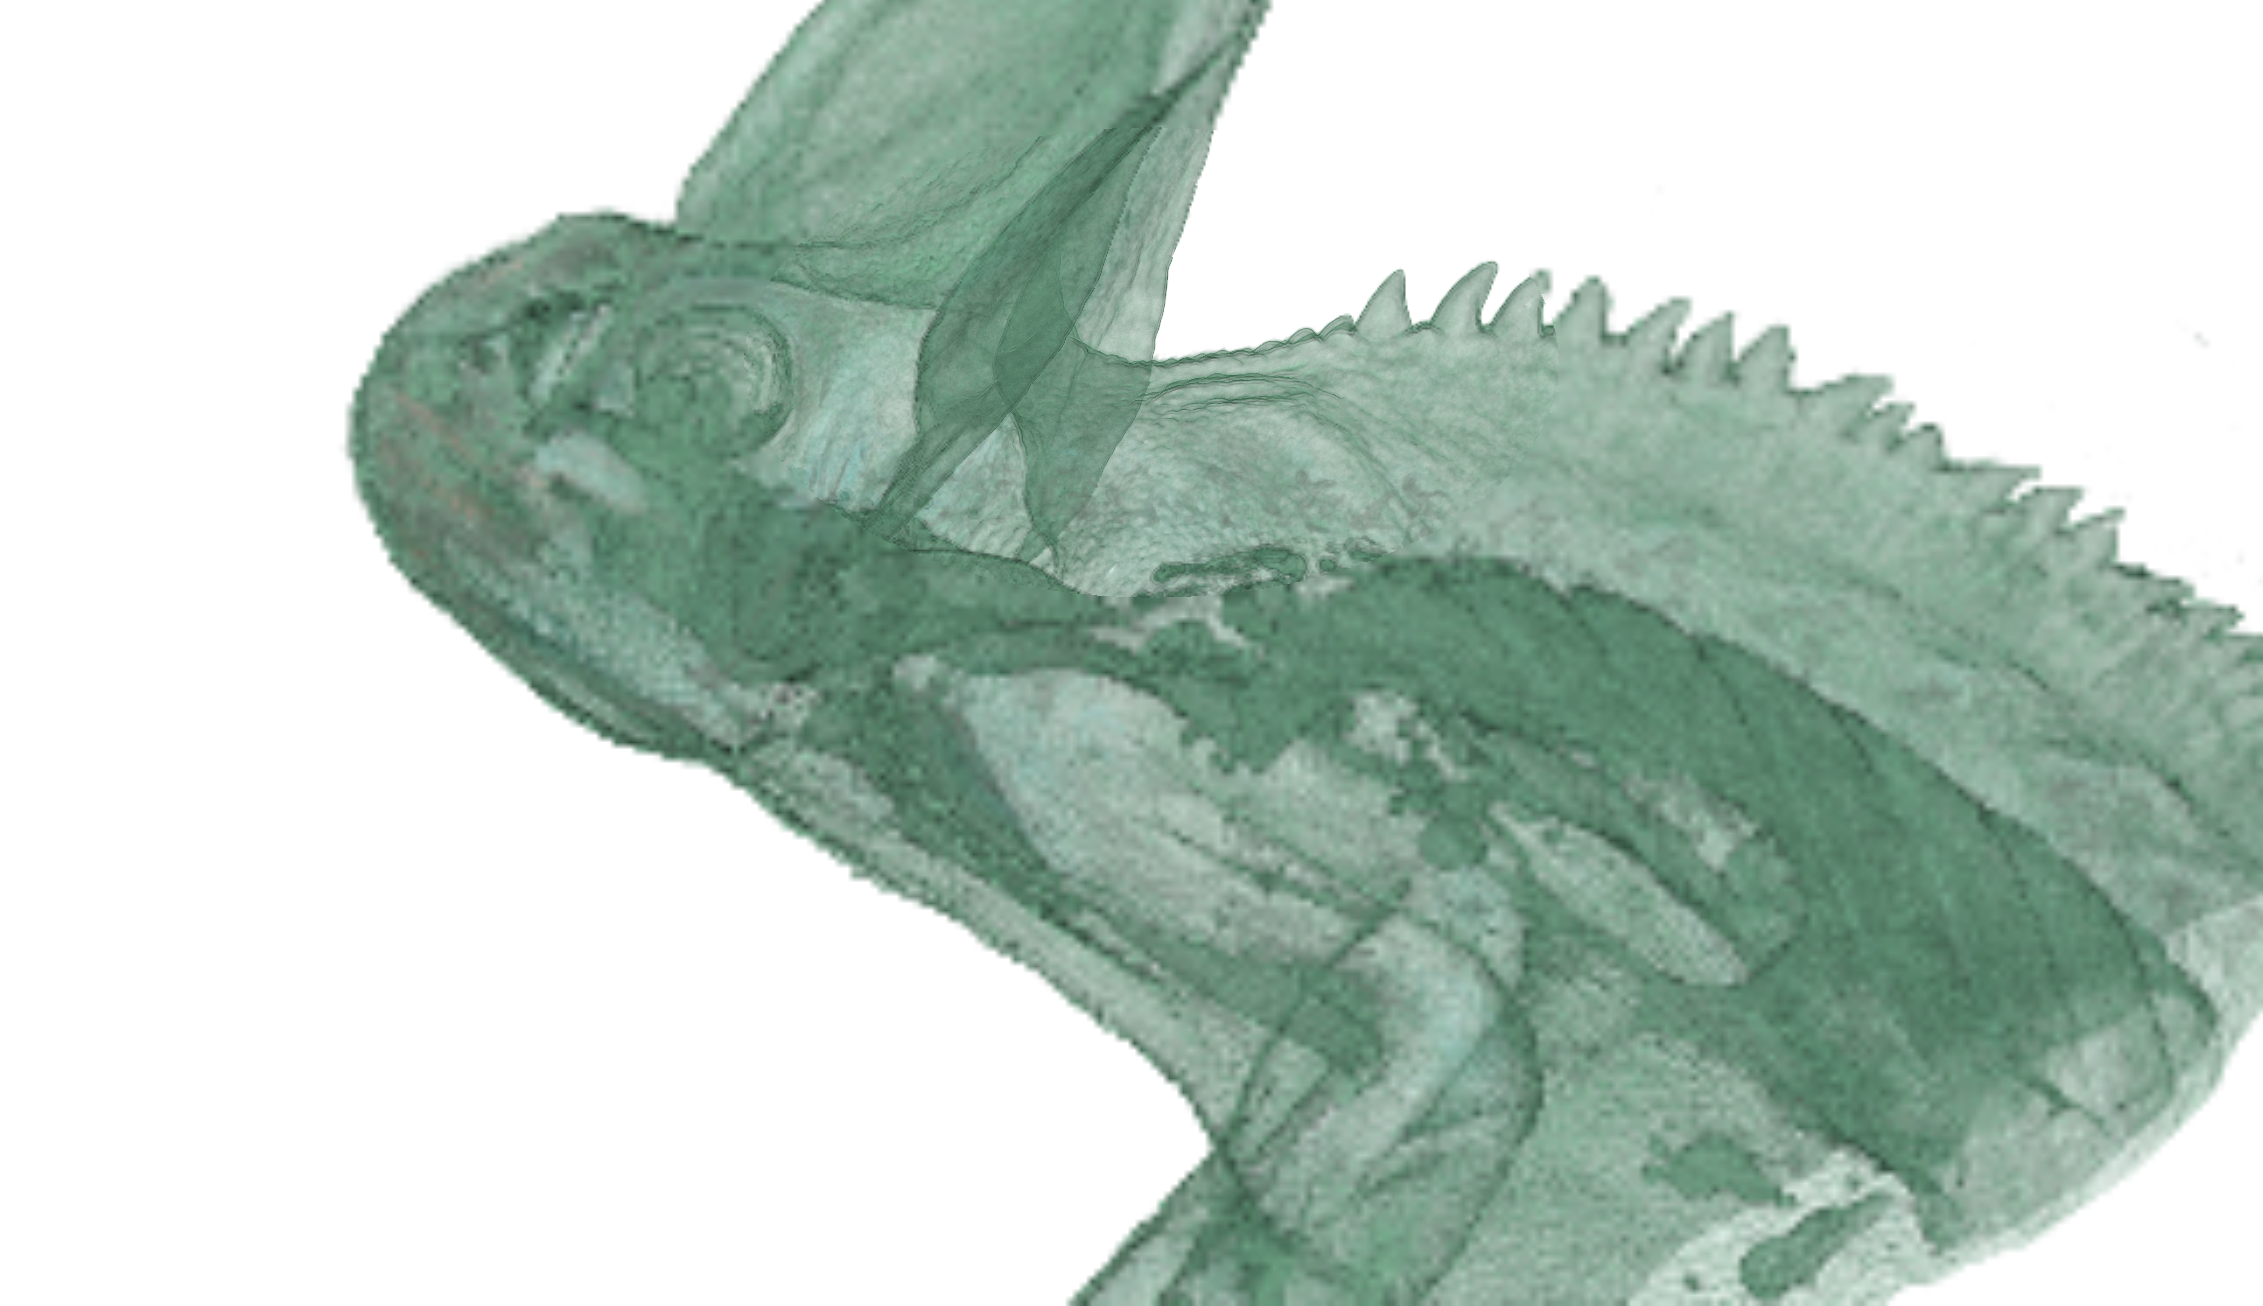
\includegraphics[width=1\textheight]{../../Grafiken/results/picture_quality/chameleon/DDC_img-1_ray-1-5.png}
		\caption{Volumen Chameleon mit \emph{DDC} Raycast berechnet.}
		\label{fig::res::cam_ddc}
	\end{figure}
\end{landscape}


\begin{landscape}
	\begin{figure}
		\centering
		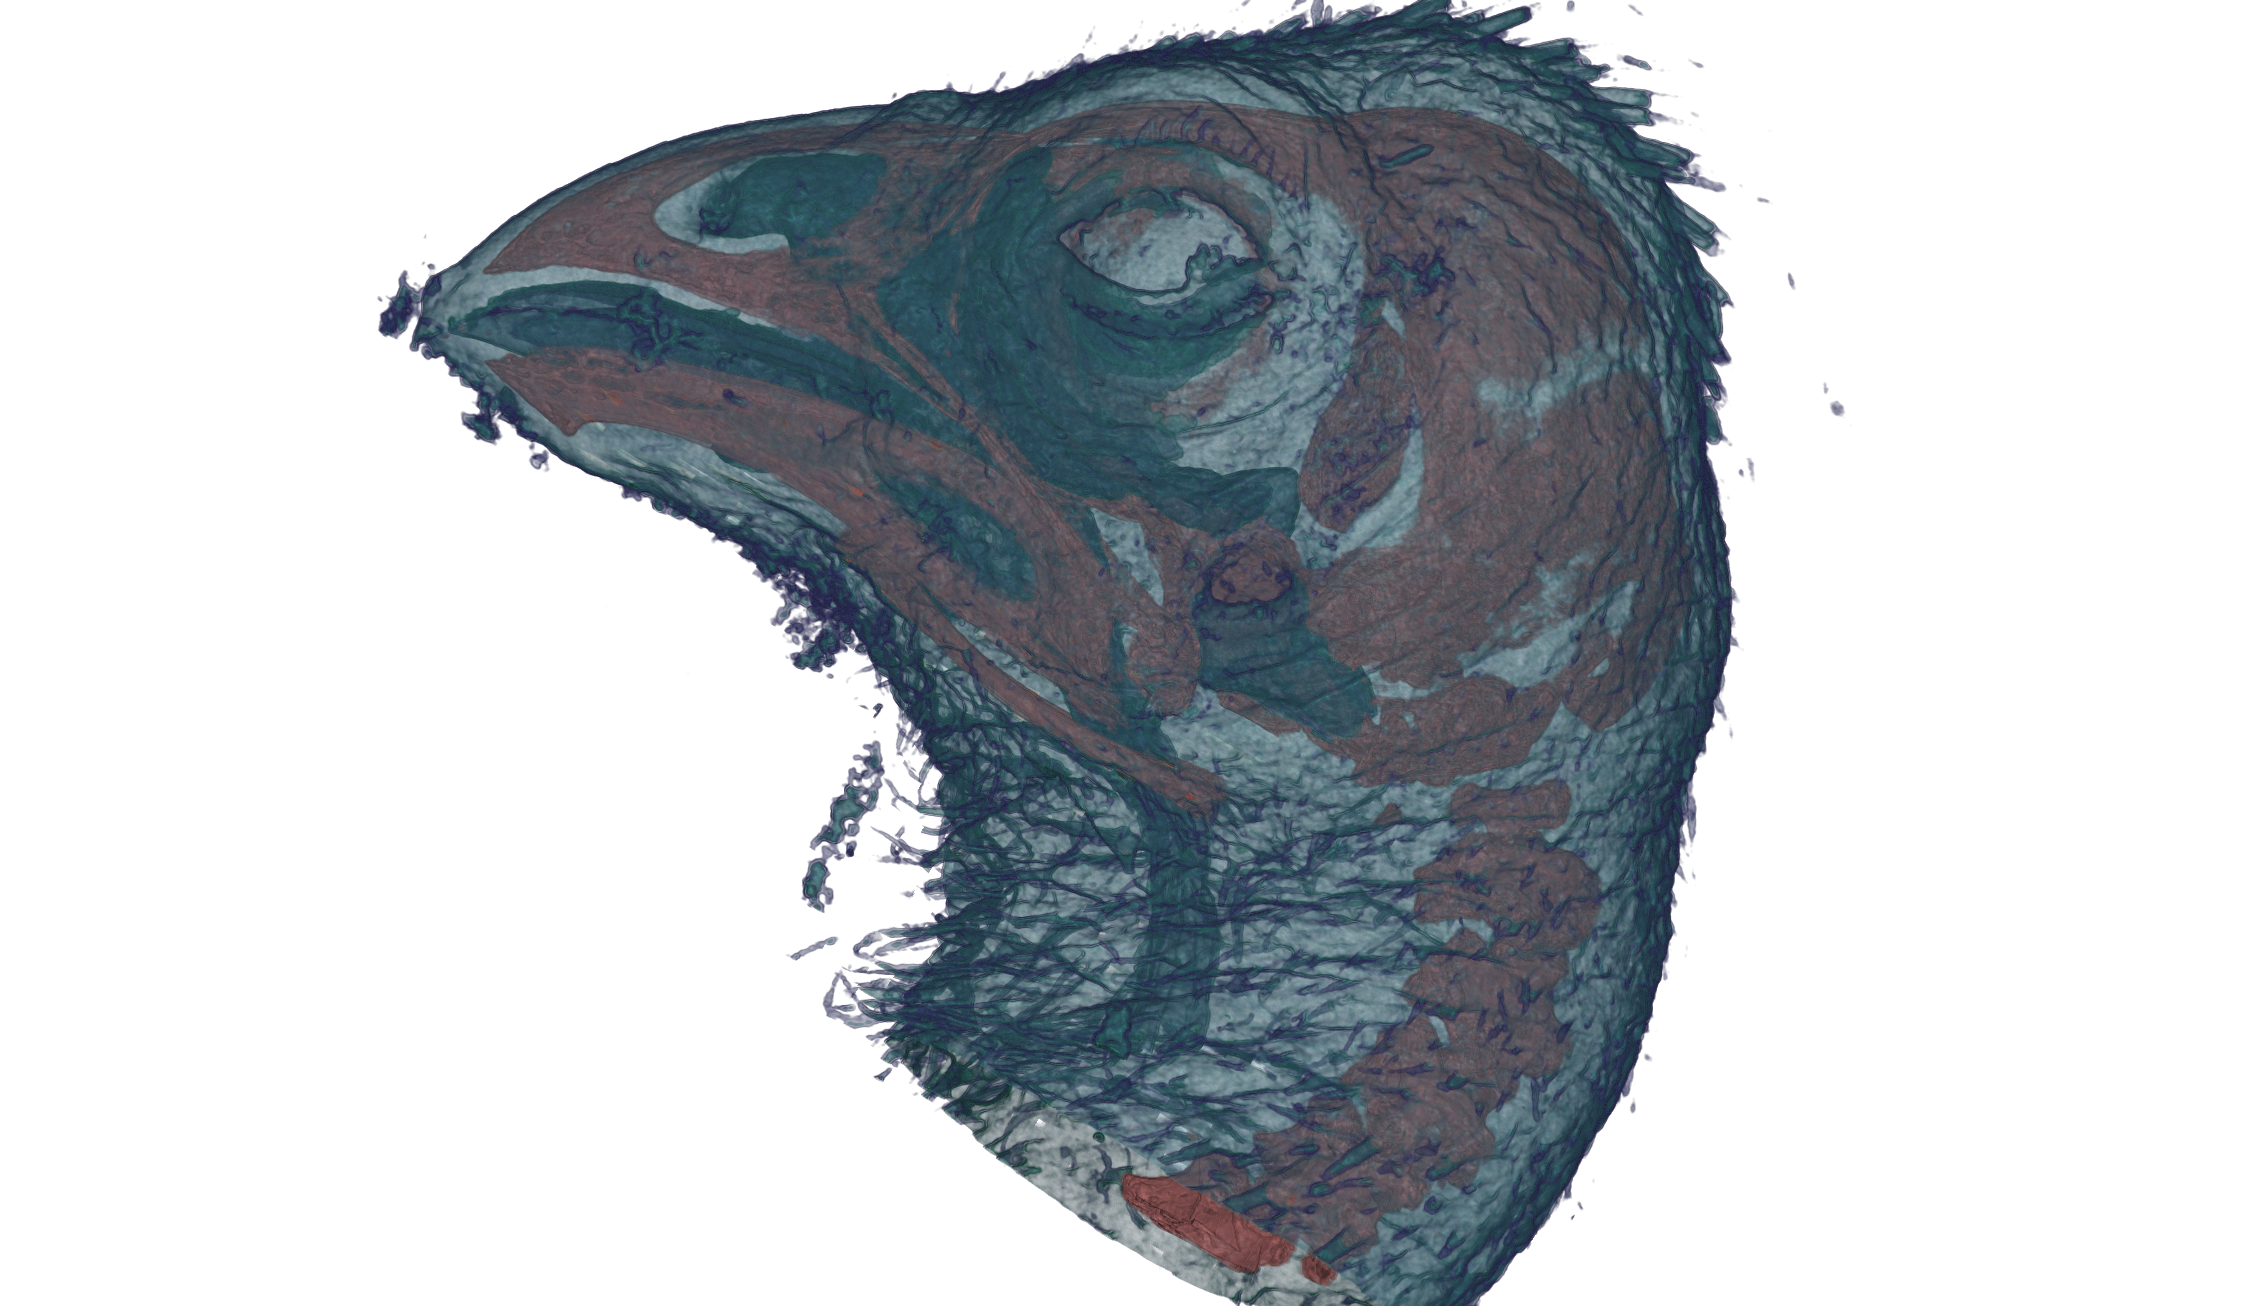
\includegraphics[width=1\textheight]{../../Grafiken/results/picture_quality/hoatzin/Standard_img-1_Ray-1-5.png}
		\caption{Volumen Hoatzin mit ursprünglichem Raycast berechnet.}
		\label{fig::res::hoa_st}
	\end{figure}
\end{landscape}

\begin{landscape}
	\begin{figure}
		\centering
		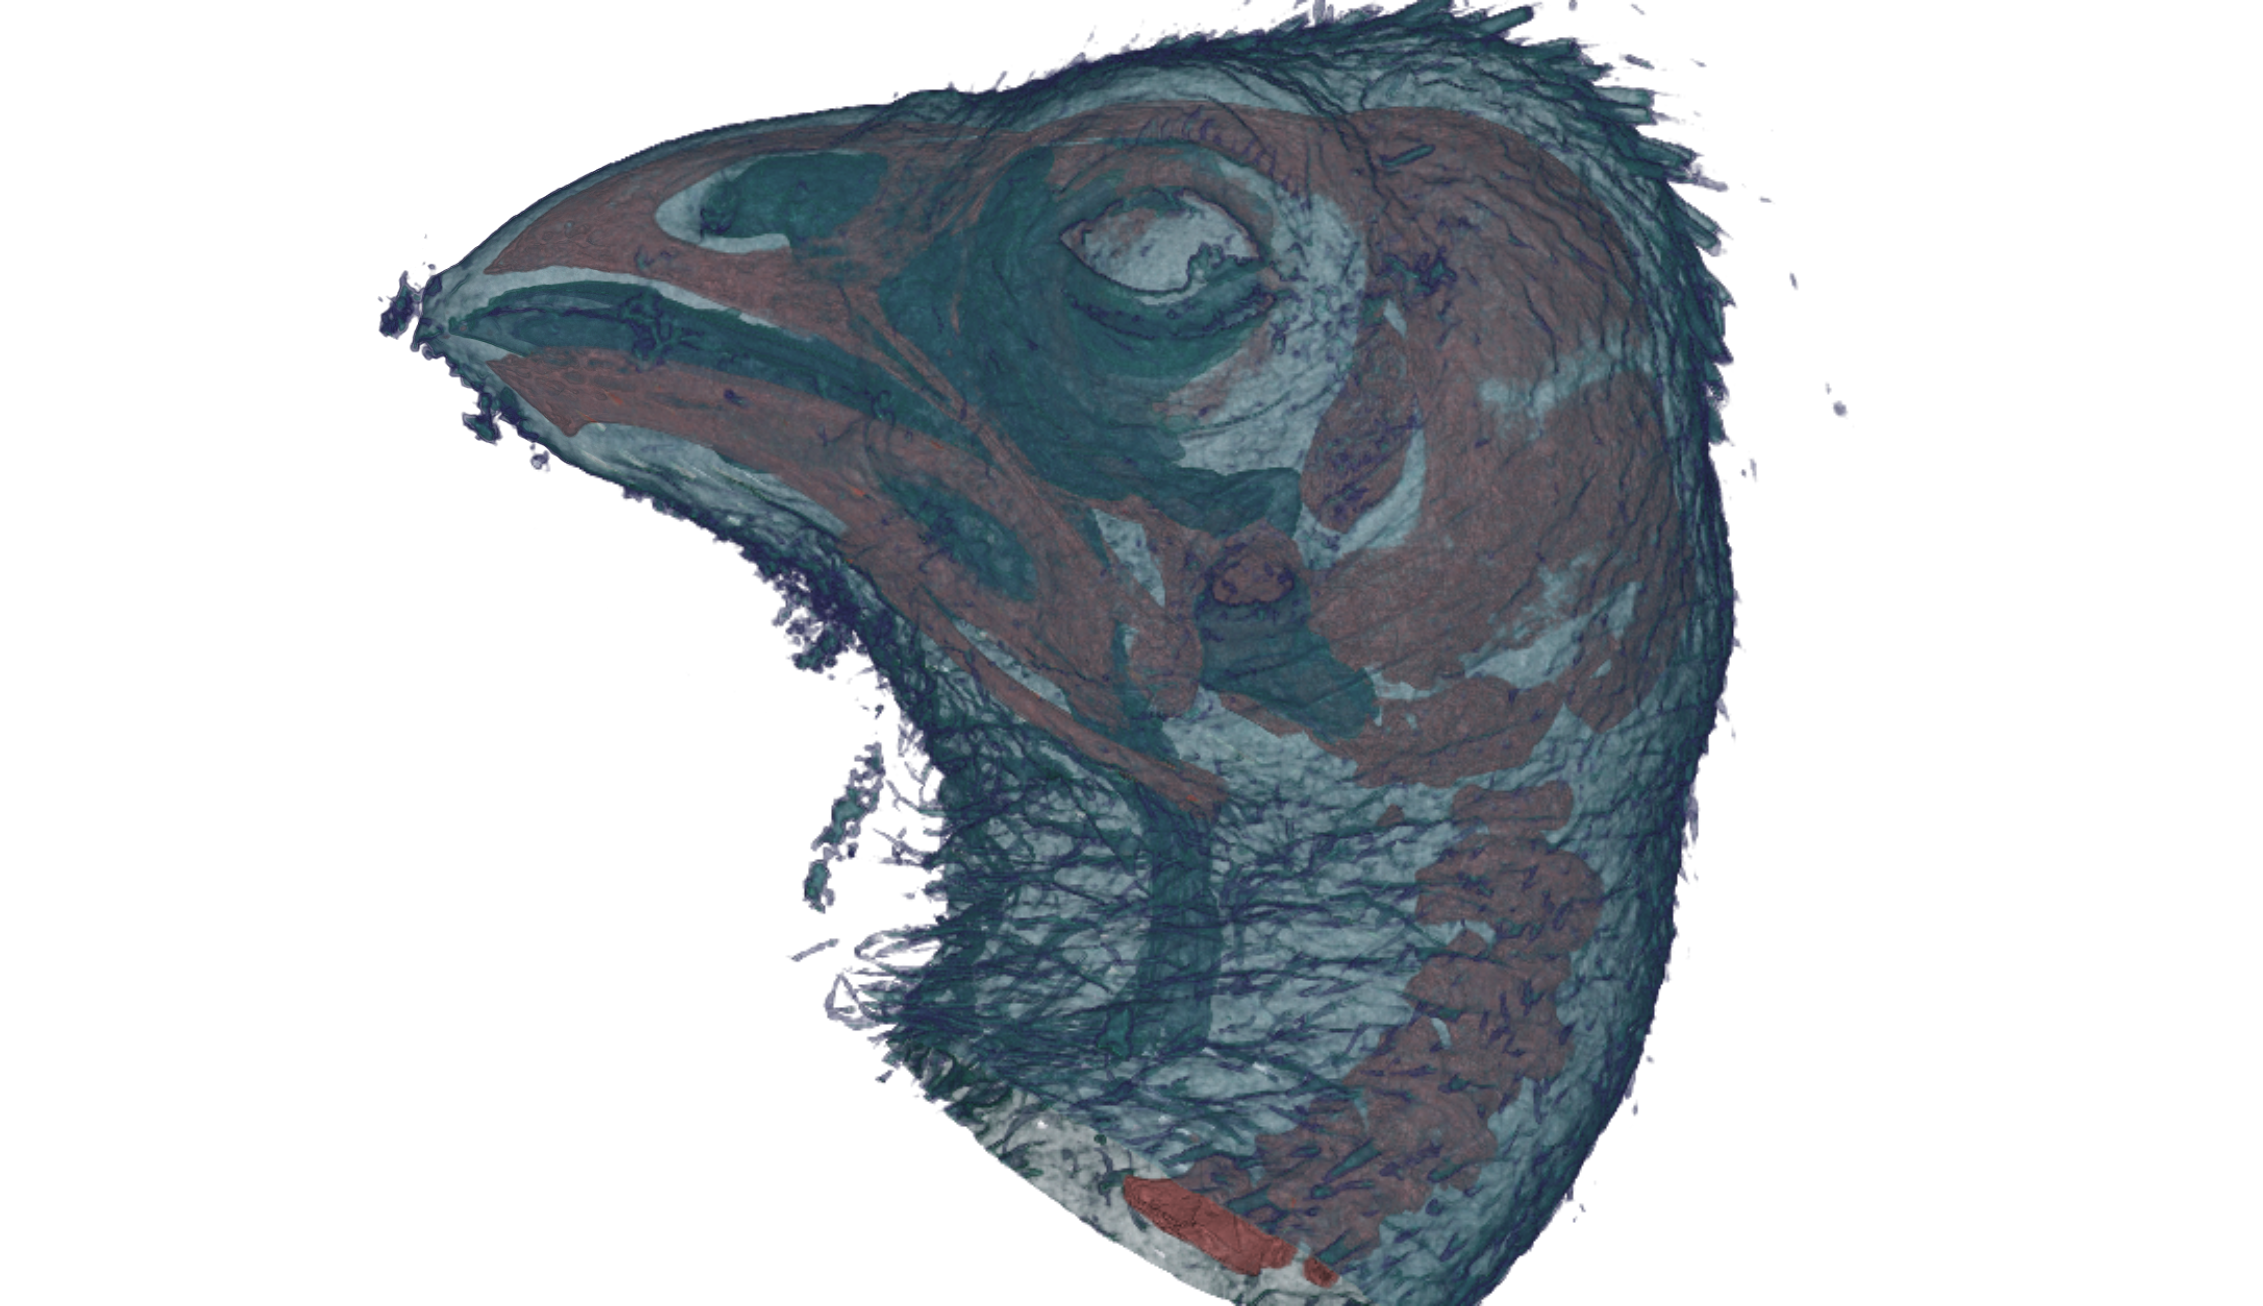
\includegraphics[width=1\textheight]{../../Grafiken/results/picture_quality/hoatzin/MDC_img-0-96_ray-1-5.png}
		\caption{Volumen Hoatzin mit \emph{MDC} Raycast berechnet.}
		\label{fig::res::hoa_mdc}
	\end{figure}
\end{landscape}

\begin{landscape}
	\begin{figure}
		\centering
		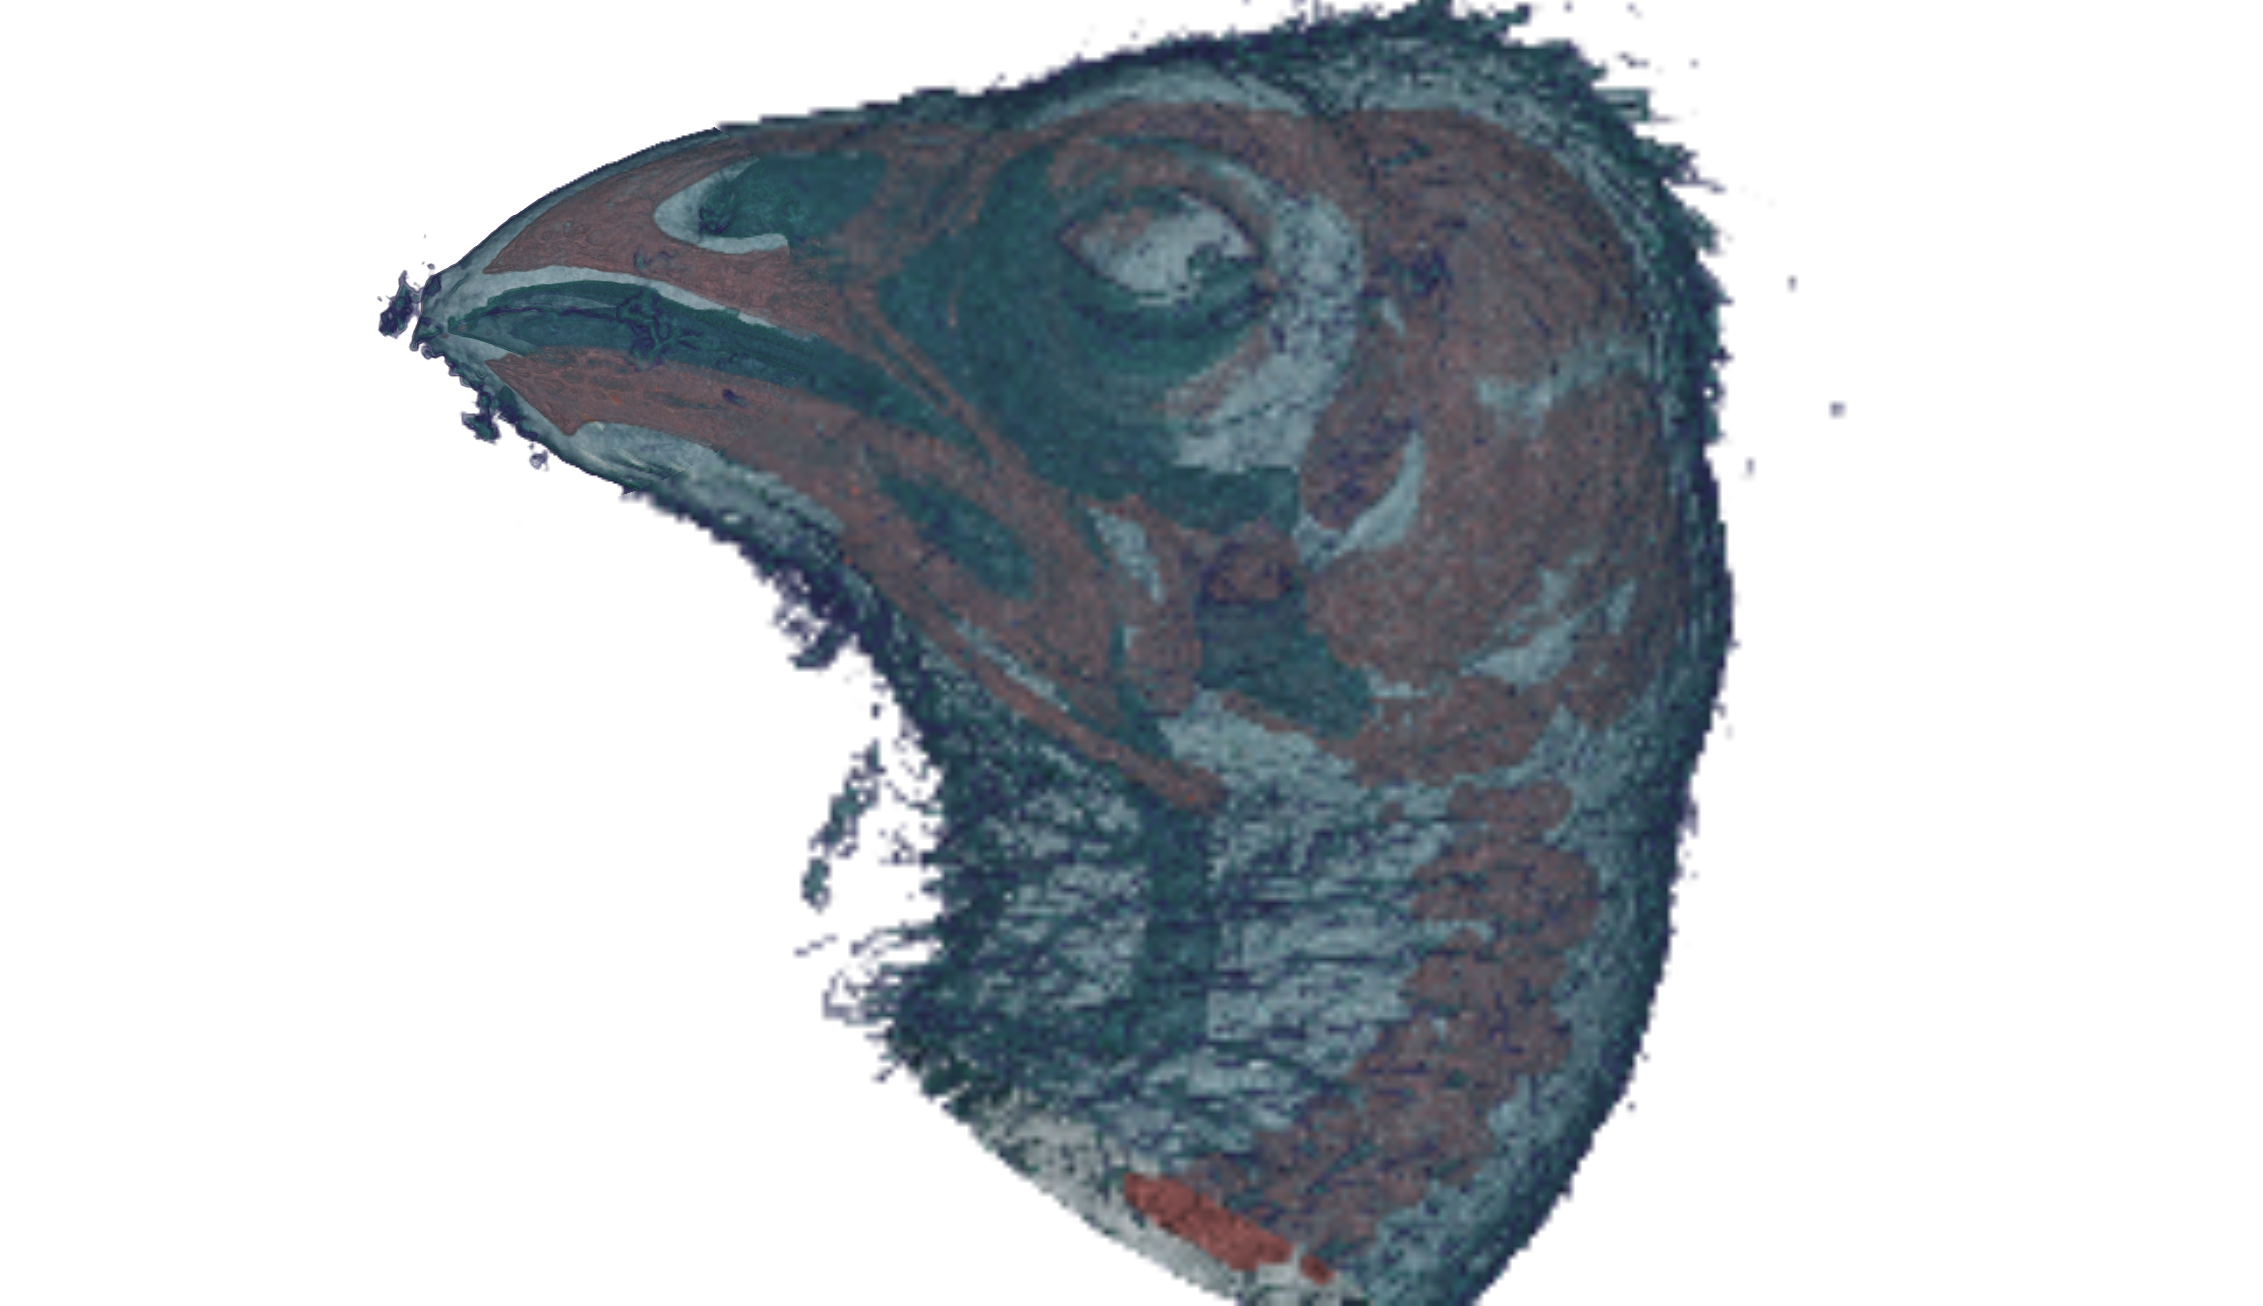
\includegraphics[width=1\textheight]{../../Grafiken/results/picture_quality/hoatzin/DDC_img-1_ray-1-5.png}
		\caption{Volumen Hoatzin mit \emph{DDC} Raycast berechnet.}
		\label{fig::res::hoa_ddc}
	\end{figure}
\end{landscape}
\fi

\subsection{Performanz}





\todo{Messbare Ergebnisse der Arbeit. (Performanzmessungen..).}

\section*{Diskussion}\label{sec::disc}
\todo{Diskussion und Bedeutung der Ergebnisse.}